\section{命題1と命題2の証明}
\label{sec:app_proofs}
\textbf{命題1．}$S\bom=D^{-1/2}WD^{-1/2}D^{1/2}\mathbf{1}=D^{-1/2}W\mathbf{1}=\bom$であり，$S$は対称なので$\bom^{\top}S=\bom^{\top}$．よって$\bom^{\top}\mathbf{u}^{(\ell+1)}=\lambda\bom^{\top}\mathbf{u}^{(\ell)}+(1-\lambda)\bom^{\top}\mathbf{y}^{+}$となり，$\mathbf{u}^{(0)}=\mathbf{0}$から解けば$\bom^{\top}\mathbf{u}^{(L)}=(1-\lambda^{L})\bom^{\top}\mathbf{y}^{+}=(1-\lambda^{L})\sum_{j\in\mathcal{S}}\sqrt{\delta_j}$を得る．$\square$

\textbf{命題4．}$\sigma$を折$b$の節点の上の関数とみる．それを定めるのは，支持画像，折$\bar b$の節点とその較正・テストの区別，および「$\mathcal{C}_b\cup\mathcal{T}_b$という節点の集合」だけである．グラフと$\mathbf{u}^{+}$は節点の名札に依らず（\secref{graph}），$\hat{Q}_{\bar b}$と$\mathbf{u}^{-}_{\bar b}$は折$\bar b$の画像と$\mathbf{u}^{+}$から決まり，参照する較正画像は$\mathcal{C}_{\bar b}$である．したがって$\sigma$は，$\mathcal{C}_b\cup\mathcal{T}_b$の中でどの節点を較正画像と呼ぶかを入れ替えても変わらない．これはAdaDetectの条件(8)（学習標本を支持画像と折$\bar b$の全節点，帰無の較正標本を$\mathcal{C}_b$，テスト標本を$\mathcal{T}_b$としたもの．同論文の証明は学習標本を所与とした置換の議論なので，その中身は問わない）であり，\eqnref{pfin}の$\pfin$は同論文の経験$p$値(10)である．よって定理3.3から(i)と(ii)のPRDS・超一様性が従い，系3.5と系3.7がFDRの上界を与える．$\square$

\textbf{系1．}\eqnref{walk}のランダムウォーク（各ステップで確率$1-\lambda$で止まる）で，$Q$から初めて外へ出る時刻を$\tau$とする．$Q\cap Y=\emptyset$なので$X_T\in Y$には$\tau\le T$が要り，止まる時刻$T$は幾何分布で無記憶だから，強マルコフ性より$u_i/\sqrt{\delta_i}=\mathbb{E}_i[\mathbf{1}[\tau\le T]\,u_{X_\tau}/\sqrt{\delta_{X_\tau}}]\le\Pr_i(\tau\le T)\max_{j\in\partial Q}u_j/\sqrt{\delta_j}$（$X_\tau\in\partial Q$）．$\pi_i=\Pr_i(\tau\le T)$は最初の1歩で分けると$\pi_i=\lambda(e_i+\sum_{j\in Q}P_{ij}\pi_j)$，すなわち$\boldsymbol{\pi}=\lambda(I-\lambda P_{QQ})^{-1}\mathbf{e}$を満たす（$\lambda P_{QQ}$のスペクトル半径は1未満）．$\pi^{*}=\max_{x\in Q}\pi_x$は$e_x\le\bar e_Q$から$\pi^{*}\le\lambda(\bar e_Q+(1-\bar e_Q)\pi^{*})$，すなわち$\pi^{*}\le\psi(\bar e_Q)$を満たす．$u^{+}_{x'}\le u^{+}_i$なら$u^{+}_{x'}\le b_i$なので，\eqnref{plp}の数え上げから第2式が従い，$\bar e_Q=0$なら$\boldsymbol{\pi}=\mathbf{0}$，$u^{+}_i=0$である．$\square$

\textbf{命題2．}$i\in Q$では$y_i=0$なので$u_i=\lambda\sum_jW_{ij}u_j/\sqrt{\delta_i\delta_j}$．両辺に$\sqrt{\delta_i}$を掛けて$Q$で足すと，$Q$の内側の辺からの寄与は$\sum_{j\in Q}(u_j/\sqrt{\delta_j})\sum_{i\in Q}W_{ij}\le\sum_{j\in Q}\sqrt{\delta_j}u_j$で抑えられ，外側の辺からの寄与は$w(Q,\bar{Q})\max_{j}u_j/\sqrt{\delta_j}$で抑えられる．\eqnref{walk}と同じランダムウォークの表現より$u_j/\sqrt{\delta_j}\le1/\min_{s\in Y}\sqrt{\delta_s}$なので，移項して\eqnref{cond}を得る．$\square$

\section{最終読み出しの保証の実測と種に混じるIDの割合}
\label{sec:app_fdp}
\secref{fdp}の2つの設定の詳細を示す．

\textbf{交換可能な較正（検証画像）．}較正画像をIDの検証画像からクラスあたり4枚取り（残りの検証画像がIDのテスト集合），支持画像は学習画像のままにすると，較正画像とIDのテスト画像は交換可能になる．\NVcalNSplits{}通りの抽出・9データセットで，IDの誤警報率$\Pr(\pfin\le\alpha)$は$\alpha{=}0.01$で\NVcalFprZeroZeroOneMin{}--\NVcalFprZeroZeroOneMax{}，$0.05$で\NVcalFprZeroZeroFiveMin{}--\NVcalFprZeroZeroFiveMax{}，$0.1$で\NVcalFprZeroOneMin{}--\NVcalFprZeroOneMax{}，$0.2$で\NVcalFprZeroTwoMin{}--\NVcalFprZeroTwoMax{}とどの水準でも$\alpha$のまわりに収まり，$\pfin$へのBH法（$q{=}0.2$）の偽発見割合は\NVcalBhFdpMin{}--\NVcalBhFdpMax{}で水準以下，その再現率（未知のうち棄却された割合）は\NVcalBhRecallMin{}--\NVcalBhRecallMax{}である．種に混じるIDの割合（折ごと，命題3の対象）も$q{=}0.2$で\NVcalIdfracStoreyMin{}--\NVcalIdfracStoreyMax{}（Storey型）である．検知性能は学習画像の較正と変わらない（near-OODの\FPR{}は$\times$TINSで\NVcalMainNearFpr\%，単体で\NVcalAloneNearFpr\%）．命題4の保証は実測でも成り立つ．

\textbf{ベンチマークの較正（学習画像）．}同じ量を\tabref{main}の設定（6通りの抽出）で測ると，$\Pr(\pfin\le0.05)$は\NVtrainFprZeroZeroFiveMin{}--\NVtrainFprZeroZeroFiveMax{}，BH法の偽発見割合は\NVtrainBhFdpMin{}--\NVtrainBhFdpMax{}，種のIDの割合は\NVtrainIdfracStoreyMin{}--\NVtrainIdfracStoreyMax{}（単純BH法では\NVtrainIdfracBhMin{}--\NVtrainIdfracBhMax{}）であり，学習画像と検証画像のずれの分だけ水準を超える（\tabref{fdp}）．ベンチマークの値（\tabref{main}）はその定めどおり学習画像の較正で報告する．


\tabref{val}に，交換可能な較正での$\pfin$の実測の誤警報率とBH法の偽発見割合をデータセット別に示す．\tabref{fdp}に，\tabref{main}の設定（学習画像の較正，$q{=}0.2$，6通りの抽出の平均）で折ごとに選ばれた種の数（2つの折の平均）と，種に混じっていたIDの割合（実測の偽発見割合）を，Storey型と単純BH法の両方について，データセット別・ビュー別に示す（\secref{fdp}）．交換可能な較正での同じ量は\secref{fdp}の本文に範囲で示した．

\begin{table}[t]
\centering
\caption{最終スコア$\pfin$の保証の実測（交換可能な較正：IDの検証画像からクラスあたり4枚を較正画像とし，\NVcalNSplits{}通りの抽出の平均，単体）．IDの誤警報率は$\pfin\le\alpha$と判定されたIDのテスト画像の割合（命題4(i)：$\le\alpha$），偽発見割合はBH法（$q{=}0.2$）で棄却された画像のうちIDの割合（命題4(ii)：期待値$\le0.2$），再現率は未知のうち棄却された割合．}
\label{tab:val}
\vspace{1.5mm}
{\fontsize{6.5pt}{7.6pt}\selectfont\renewcommand{\arraystretch}{1.0}%
\setlength{\tabcolsep}{1.7pt}\begin{tabular}{@{}lcccc|cc@{}}
\hline
\rule[-2.0pt]{0pt}{8.6pt} & \multicolumn{4}{c|}{IDの誤警報率 $\Pr(\pfin\le\alpha)$} & \multicolumn{2}{c}{BH法（$q{=}0.2$）} \\
\rule[-2.0pt]{0pt}{8.6pt}データセット & $\alpha{=}0.01$ & $0.05$ & $0.1$ & $0.2$ & 偽発見割合 & 再現率 \\
\hline
SSB-hard & 0.009 & 0.051 & 0.099 & 0.201 & 0.091 & 0.901 \\
NINCO & 0.011 & 0.052 & 0.100 & 0.197 & 0.183 & 0.983 \\
iNaturalist & 0.009 & 0.049 & 0.099 & 0.198 & 0.158 & 0.998 \\
Textures & 0.011 & 0.054 & 0.103 & 0.202 & 0.191 & 0.928 \\
OpenImage-O & 0.009 & 0.051 & 0.103 & 0.199 & 0.147 & 0.901 \\
iNat. (Four-OOD) & 0.009 & 0.050 & 0.101 & 0.203 & 0.165 & 0.998 \\
SUN & 0.010 & 0.051 & 0.097 & 0.200 & 0.168 & 0.981 \\
Places & 0.009 & 0.050 & 0.099 & 0.198 & 0.165 & 0.855 \\
Textures (Four-OOD) & 0.011 & 0.051 & 0.102 & 0.203 & 0.191 & 0.915 \\
\hline
\end{tabular}}%

\end{table}

\begin{table}[t]
\centering
\caption{学習画像の較正で選ばれた種（折あたり，6通りの抽出の平均）．種は種の数，ID率は種に混じっていたIDの割合（実測の偽発見割合，水準$q{=}0.2$）．}
\label{tab:fdp}
\vspace{1.5mm}
{\fontsize{6.0pt}{7.1pt}\selectfont\renewcommand{\arraystretch}{1.0}%
\setlength{\tabcolsep}{1.3pt}\begin{tabular}{@{}lcccc|cccc@{}}
\hline
\rule[-2.0pt]{0pt}{8.2pt} & \multicolumn{4}{c|}{DINOv2 L/14} & \multicolumn{4}{c}{DINOv3 L/16} \\
\rule[-2.0pt]{0pt}{8.2pt} & \multicolumn{2}{c}{Storey型} & \multicolumn{2}{c|}{単純BH} & \multicolumn{2}{c}{Storey型} & \multicolumn{2}{c}{単純BH} \\
\rule[-2.0pt]{0pt}{8.2pt}データセット & 種 & ID率 & 種 & ID率 & 種 & ID率 & 種 & ID率 \\
\hline
SSB-hard & 30,383 & 0.219 & 23,993 & 0.102 & 31,030 & 0.230 & 24,227 & 0.103 \\
NINCO & 3,784 & 0.254 & 3,597 & 0.219 & 3,993 & 0.281 & 3,685 & 0.226 \\
iNaturalist & 6,642 & 0.249 & 6,197 & 0.196 & 6,808 & 0.266 & 6,240 & 0.200 \\
Textures & 3,064 & 0.248 & 2,892 & 0.213 & 3,277 & 0.278 & 3,030 & 0.230 \\
OpenImage-O & 9,433 & 0.235 & 8,281 & 0.167 & 9,932 & 0.256 & 8,584 & 0.174 \\
iNat. (Four-OOD) & 6,653 & 0.250 & 6,235 & 0.201 & 6,895 & 0.276 & 6,326 & 0.211 \\
SUN & 6,414 & 0.249 & 5,911 & 0.192 & 6,668 & 0.266 & 6,075 & 0.199 \\
Places & 5,587 & 0.246 & 5,071 & 0.196 & 5,960 & 0.260 & 5,313 & 0.196 \\
Textures (Four-OOD) & 3,325 & 0.255 & 3,103 & 0.214 & 3,492 & 0.272 & 3,253 & 0.230 \\
\hline
\end{tabular}}%

\end{table}

\section{データセット別の値と散布図}
\label{sec:app_four}
\tabref{perds}と\tabref{four}に\tabref{main}のデータセット別の値を示す（\secref{main}）．\figref{scatter}は\tabref{main}の全手法の\AUC{}と\FPR{}の散布図である．

\begin{table*}[t]
\centering
\caption{OpenOOD v1.5 ImageNet-1Kのデータセット別の結果（[\%]，AUROC$\uparrow$／FPR95$\downarrow$）．記法は\tabref{main}と同じ．TINSの報告値は原論文の表8のとおりで，iNaturalistとTexturesは同論文のFour-OODの表1と同じ値が報告されている（\tabref{four}）．}
\label{tab:perds}
\vspace{1.5mm}
{\fontsize{7pt}{8.2pt}\selectfont\renewcommand{\arraystretch}{1.0}%
\setlength{\tabcolsep}{2.0pt}\begin{tabular}{@{}lcccccccccc@{}}
\hline
\rule[-2.0pt]{0pt}{8.6pt} & \multicolumn{4}{c}{near-OOD} & \multicolumn{6}{c}{far-OOD} \\
\rule[-2.0pt]{0pt}{8.6pt} & \multicolumn{2}{c}{SSB-hard} & \multicolumn{2}{c}{NINCO} & \multicolumn{2}{c}{iNaturalist} & \multicolumn{2}{c}{Textures} & \multicolumn{2}{c}{OpenImage-O} \\
\rule[-2.0pt]{0pt}{8.6pt}手法 & AUROC & FPR95 & AUROC & FPR95 & AUROC & FPR95 & AUROC & FPR95 & AUROC & FPR95 \\
\hline
MOODv2~\cite{li2024moodv2}$^{\dagger}$ & 85.00 & 58.10 & 92.70 & 38.20 & 99.60 & 1.80 & 94.30 & 24.70 & 97.40 & 13.60 \\
NNGuide~\cite{park2023nnguide}$^{\dagger}$ & 84.70 & 54.70 & 93.70 & 28.90 & 99.90 & 1.80 & 95.80 & 17.00 & 97.70 & 10.80 \\
RankFeat~\cite{song2022rankfeat}$^{\dagger}$ & 89.40 & 47.90 & 90.00 & 39.30 & 96.00 & 13.00 & 95.00 & 25.40 & 92.40 & 33.30 \\
SCALE~\cite{xu2024scale}$^{\dagger}$ & 77.40 & 67.70 & 85.40 & 51.80 & 98.00 & 9.50 & 97.60 & 11.90 & 94.00 & 28.20 \\
DisCoPatch~\cite{caetano2025discopatch}$^{\dagger}$ & 95.80 & 19.80\sota & 94.30 & 39.00 & 99.10 & 3.60 & 96.40 & 18.90 & 94.40 & 29.70 \\
TINS~\cite{yang2026tins}$^{\dagger}$ & 81.38 & 61.68 & 83.91 & 54.09 & 99.93 & 0.21 & 97.83 & 10.09 & 92.99 & 28.68 \\
TINS~\cite{yang2026tins}（実測） & 82.22 & 56.65 & 80.74 & 56.09 & 99.93 & 0.17 & 98.11 & 8.31 & 93.09 & 28.20 \\
Salmon Ladder，単体 & \cellcolor{upd}\textbf{96.24} & 21.72 & \cellcolor{upd}\textbf{99.65} & \cellcolor{upd}\textbf{1.28} & 99.93 & \cellcolor{upd}\textbf{0.16} & \cellcolor{upd}\textbf{98.91} & \cellcolor{upd}\textbf{4.37} & 97.55 & 10.98 \\
Salmon Ladder $\times$TINS & \cellcolor{upd}\textbf{96.51}\sota & 19.96 & \cellcolor{upd}\textbf{99.68}\sota & \cellcolor{upd}\textbf{1.03}\sota & \cellcolor{upd}\textbf{99.96}\sota & \cellcolor{upd}\textbf{0.11}\sota & \cellcolor{upd}\textbf{99.31}\sota & \cellcolor{upd}\textbf{2.56}\sota & \cellcolor{upd}\textbf{97.87}\sota & \cellcolor{upd}\textbf{9.81}\sota \\
{\scriptsize\textcolor{black!60}{\quad 最良の比較手法との差}} & \gap{+0.71} & \gap{-0.16} & \gap{+5.38} & \gap{+27.87} & \gap{+0.03} & \gap{+0.06} & \gap{+1.20} & \gap{+5.75} & \gap{+0.17} & \gap{+0.99} \\
\hline
\end{tabular}}%

\end{table*}

\begin{figure*}[t]
\centering
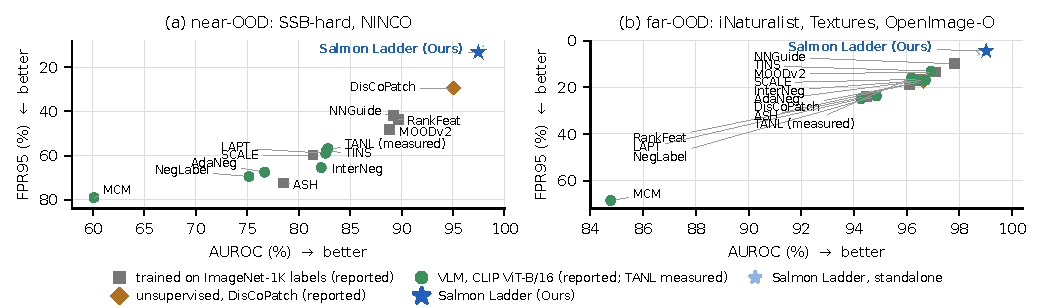
\includegraphics[width=\textwidth]{figs/fig18_scatter.pdf}
\caption{OpenOOD v1.5 ImageNet-1Kでの\AUC{}と\FPR{}（\tabref{main}の全手法，右上ほど良い）．大きな星が本稿の構成（$\times$TINS），小さな星は単体．比較手法は報告値（TANLのみ実測）．}
\label{fig:scatter}
\end{figure*}

\begin{table*}[t]
\centering
\caption{Four-OOD（ImageNet-1Kに対するiNaturalist，SUN，Places，Textures，[\%]）．比較手法はすべてCLIP ViT-B/16による報告値$\dagger$（TINSは実測も併記）．記法は\tabref{main}と同じ．}
\label{tab:four}
\vspace{1.5mm}
{\fontsize{7pt}{8.2pt}\selectfont\renewcommand{\arraystretch}{1.0}%
\setlength{\tabcolsep}{2.0pt}\begin{tabular}{@{}lcccccccccc@{}}
\hline
\rule[-2.0pt]{0pt}{8.6pt} & \multicolumn{2}{c}{iNaturalist} & \multicolumn{2}{c}{SUN} & \multicolumn{2}{c}{Places} & \multicolumn{2}{c}{Textures} & \multicolumn{2}{c}{平均} \\
\rule[-2.0pt]{0pt}{8.6pt}手法 & AUROC & FPR95 & AUROC & FPR95 & AUROC & FPR95 & AUROC & FPR95 & AUROC & FPR95 \\
\hline
MCM~\cite{ming2022mcm}$^{\dagger}$ & 94.59 & 32.20 & 92.25 & 38.80 & 90.31 & 46.20 & 86.12 & 58.50 & 90.82 & 43.93 \\
NegLabel~\cite{jiang2024neglabel}$^{\dagger}$ & 99.49 & 1.91 & 95.49 & 20.53 & 91.64 & 35.59 & 90.22 & 43.56 & 94.21 & 25.40 \\
CSP~\cite{chen2024csp}$^{\dagger}$ & 99.60 & 1.54 & 96.66 & 13.66 & 92.90 & 29.32 & 93.86 & 25.52 & 95.76 & 17.51 \\
OODD~\cite{yang2025oodd}$^{\dagger}$ & 99.79 & 0.85 & 97.17 & 12.94 & 92.51 & 30.68 & 94.51 & 30.67 & 96.00 & 18.79 \\
AdaNeg~\cite{zhang2024adaneg}$^{\dagger}$ & 99.71 & 0.59 & 97.44 & 9.50 & 94.55 & 34.34 & 94.93 & 31.27 & 96.66 & 18.92 \\
InterNeg~\cite{xu2026interneg}$^{\dagger}$ & 99.79 & 0.40 & 98.68 & 6.78 & 95.01 & 27.11 & 96.26 & 21.85 & 97.43 & 14.04 \\
TINS~\cite{yang2026tins}$^{\dagger}$ & 99.93 & 0.21 & 99.14 & 3.84 & 97.14 & 12.73 & 97.83 & 10.09 & 98.51 & 6.72 \\
TINS~\cite{yang2026tins}（実測） & 99.93 & 0.22 & 99.12 & 4.35 & 97.12 & 12.98 & 97.94 & 9.83 & 98.52 & 6.85 \\
Salmon Ladder，単体 & 99.92 & \cellcolor{upd}\textbf{0.16} & \cellcolor{upd}\textbf{99.49} & \cellcolor{upd}\textbf{1.63} & 97.05 & \cellcolor{upd}\textbf{11.35} & \cellcolor{upd}\textbf{98.72} & \cellcolor{upd}\textbf{5.12} & \cellcolor{upd}\textbf{98.80} & \cellcolor{upd}\textbf{4.56} \\
Salmon Ladder $\times$TINS & \cellcolor{upd}\textbf{99.96}\sota & \cellcolor{upd}\textbf{0.11}\sota & \cellcolor{upd}\textbf{99.66}\sota & \cellcolor{upd}\textbf{0.97}\sota & \cellcolor{upd}\textbf{97.55}\sota & \cellcolor{upd}\textbf{9.26}\sota & \cellcolor{upd}\textbf{99.18}\sota & \cellcolor{upd}\textbf{3.20}\sota & \cellcolor{upd}\textbf{99.09}\sota & \cellcolor{upd}\textbf{3.39}\sota \\
{\scriptsize\textcolor{black!60}{\quad 最良の比較手法との差}} & \gap{+0.03} & \gap{+0.10} & \gap{+0.52} & \gap{+2.87} & \gap{+0.41} & \gap{+3.47} & \gap{+1.24} & \gap{+6.63} & \gap{+0.57} & \gap{+3.33} \\
\hline
\end{tabular}}%

\end{table*}

\section{ImageNet-200とCIFAR-100}
\label{sec:app_in200}
\tabref{in200}と\tabref{cifar}に\secref{in200}のImageNet-200とCIFAR-100の値を示す．CIFAR-100のIDの誤警報率$\Pr(\pfin\le0.05)$は\NCifarValNearFprZeroZeroFive{}（near）／\NCifarValFarFprZeroZeroFive{}（far），BH法の偽発見割合は\NCifarValNearBhfdp{}／\NCifarValFarBhfdp{}である（学習画像の較正）．CIFAR-100の$32\times32$の画像は他と同じ前処理で拡大して入力し，TexturesはImageNet-1Kベンチマークと同じ画像ファイルなので特徴を共有する．CIFAR-100の種は，Storey型$q{=}0.2$でCIFAR-10・Tiny ImageNetでは折の\NCifarSeedNearStoreyRatioMin{}--\NCifarSeedNearStoreyRatioMax\%，MNIST・SVHN・Places365では\NCifarSeedFarHiStoreyRatioMin{}--\NCifarSeedFarHiStoreyRatioMax\%，Texturesでは\NCifarSeedTextureStoreyRatio\%を占め，種に混じるIDの割合は\NCifarSeedStoreyIdfracMin{}--\NCifarSeedStoreyIdfracMax{}である（DINOv3 L/16のビュー，2つの折・6通りの抽出の平均）．単純BH法の種は折の\NCifarSeedTextureBhRatio{}--\NCifarSeedMnistBhRatio\%，IDの割合\NCifarSeedMnistBhIdfrac{}--\NCifarSeedTinBhIdfrac{}である．種に混じるIDの割合は命題3どおり$q$以下でも，割合$q$の種がIDのほぼ全数になって$\pN$は情報を失う（Places365：$\sigma$ \NCifarMainPlacesThreeSixFiveFpr\%，$\pP$だけ\NCifarLpPlacesThreeSixFiveFpr\%，単純BH法の種で\NCifarBhPlacesThreeSixFiveFpr\%，上限付きの種で\NCifarStoreycPlacesThreeSixFiveFpr\%）．ImageNet-200のSSB-hardでは未知が全画像の\NInTwoZeroZeroMixSsbHard\%を占めてStorey型の$\hat{\pi}_0$が\NInTwoZeroZeroSeedSsbHardStoreyPiZero{}になり，水準$q/\hat{\pi}_0$が1を超えて折の全画像が種になる（単純BH法の種は折の\NInTwoZeroZeroSeedSsbHardBhRatioPct\%，上限付きの種は\NInTwoZeroZeroSeedSsbHardStoreycRatioPct\%，IDの割合\NInTwoZeroZeroSeedSsbHardStoreycIdfrac{}）．

\begin{table}[t]
\centering
\caption{OpenOOD v1.5 CIFAR-100（[\%]，単体，\NCifarNDraws{}通りの抽出の平均）．$\dagger$はOpenOOD v1.5~\cite{zhang2023openood}の報告値（\AUC{}は論文の表2，\FPR{}は同論文の脚注6が指す公開の表）．全学習画像のkNN・クラス平均は本稿と同じ2つの特徴（L2正規化して連結），ゼロショットはCLIP ViT-B/16（\secref{in200}）．上限付きの種は$\tau{=}0.05$（\secref{cap}）．\textcolor{sotacol}{$\bigstar$}は列の最良値，\colorbox{upd}{青}は本手法以外の全行（報告値，全学習画像・ゼロショットの基線，静的検出器，LGC-max）を上回る値．}
\label{tab:cifar}
\vspace{1.5mm}
{\fontsize{6.8pt}{8pt}\selectfont\renewcommand{\arraystretch}{1.0}%
\setlength{\tabcolsep}{2pt}\begin{tabular}{@{}lcccc@{}}
\hline
\rule[-2.0pt]{0pt}{8.6pt} & \multicolumn{2}{c}{near-OOD} & \multicolumn{2}{c}{far-OOD} \\
\rule[-2.0pt]{0pt}{8.6pt}手法 & AUROC$\uparrow$ & FPR95$\downarrow$ & AUROC$\uparrow$ & FPR95$\downarrow$ \\
\hline
\multicolumn{5}{@{}l}{\rule{0pt}{6.6pt}\textit{CIFAR-100で学習したResNet-18（報告値$^{\dagger}$）}} \\
MSP$^{\dagger}$ & 80.27 & 54.80 & 77.76 & 58.70 \\
MLS$^{\dagger}$ & 81.05 & 55.47 & 79.67 & 56.73 \\
RMDS$^{\dagger}$ & 80.15 & 55.46 & 82.92 & 52.81 \\
VOS$^{\dagger}$ & 80.93 & 55.56 & 81.32 & 53.70 \\
G-ODIN$^{\dagger}$ & 77.15 & 67.58 & 85.67 & 42.68 \\
RotPred$^{\dagger}$ & 76.43 & 62.58 & 88.40 & 34.50 \\
OE$^{\dagger}$（外れ値データで学習） & 88.30 & 30.73 & 81.41 & 54.82 \\
\multicolumn{5}{@{}l}{\rule{0pt}{6.6pt}\textit{全学習画像（50,000枚）またはゼロショット（本稿で実測）}} \\
kNN，全学習画像（$k{=}50$） & 97.09 & 16.35 & 94.94 & 32.15 \\
クラス平均，全学習画像 & 97.61 & 12.91 & 95.38 & 28.05 \\
MCM~\cite{ming2022mcm}，ゼロショット & 70.30 & 94.06 & 74.59 & 89.10 \\
NegLabel~\cite{jiang2024neglabel}，ゼロショット & 72.98 & 76.98 & 80.25 & 64.84 \\
\multicolumn{5}{@{}l}{\rule{0pt}{6.6pt}\textit{凍結特徴，クラスあたり16枚，学習なし，単体（6通りの抽出の平均）}} \\
静的$p$（グラフなし） & 96.94 & 16.49 & 94.88 & 29.19 \\
kNN（グラフなし） & 92.35 & 39.22 & 88.47 & 49.80 \\
LGC-max & 98.80 & 5.39 & 99.42 & 2.21 \\
$\pP$のみ & \cellcolor{upd}\textbf{99.11} & \cellcolor{upd}\textbf{2.88} & \cellcolor{upd}\textbf{99.57} & \cellcolor{upd}\textbf{1.22} \\
$\pP\pN$，交差適合なし & \cellcolor{upd}\textbf{99.25} & \cellcolor{upd}\textbf{2.83} & 99.35 & 2.58 \\
$\sigma$（本稿の構成） & \cellcolor{upd}\textbf{99.18} & \cellcolor{upd}\textbf{2.90} & 99.37 & 2.34 \\
$\sigma$に静的$p$を加える & \cellcolor{upd}\textbf{99.34}\sota & \cellcolor{upd}\textbf{2.60} & \cellcolor{upd}\textbf{99.64}\sota & \cellcolor{upd}\textbf{1.00}\sota \\
$\sigma$，DINOv3 L/16のみ & \cellcolor{upd}\textbf{98.95} & \cellcolor{upd}\textbf{3.77} & 99.15 & 3.48 \\
$\sigma$，上限付きの種（Storey型） & \cellcolor{upd}\textbf{99.26} & \cellcolor{upd}\textbf{2.55}\sota & \cellcolor{upd}\textbf{99.59} & \cellcolor{upd}\textbf{1.46} \\
$\sigma$，上限付きの種（単純BH法） & \cellcolor{upd}\textbf{99.26} & \cellcolor{upd}\textbf{2.55}\sota & \cellcolor{upd}\textbf{99.59} & \cellcolor{upd}\textbf{1.46} \\
\hline
\end{tabular}}%

\end{table}


\begin{table}[t]
\centering
\caption{OpenOOD v1.5 ImageNet-200（[\%]，単体，\NInTwoZeroZeroNDraws{}通りの抽出の平均）．$\dagger$はOpenOOD v1.5~\cite{zhang2023openood}の報告値（ImageNet-200で学習したResNet-18；リーダーボードと同論文の脚注6が指す公開の表）．全学習画像のkNN・クラス平均は本稿と同じ2つの特徴，ゼロショットはCLIP ViT-B/16（\secref{in200}）．上限付きの種は$\tau{=}0.05$（\secref{cap}）．\textcolor{sotacol}{$\bigstar$}は列の最良値，\colorbox{upd}{青}は本手法以外の全行（報告値，全学習画像・ゼロショットの基線，静的検出器，LGC-max）を上回る値．}
\label{tab:in200}
\vspace{1.5mm}
{\fontsize{6.8pt}{8pt}\selectfont\renewcommand{\arraystretch}{1.0}%
\setlength{\tabcolsep}{2pt}\begin{tabular}{@{}lcccc@{}}
\hline
\rule[-2.0pt]{0pt}{8.6pt} & \multicolumn{2}{c}{near-OOD} & \multicolumn{2}{c}{far-OOD} \\
\rule[-2.0pt]{0pt}{8.6pt}手法 & AUROC$\uparrow$ & FPR95$\downarrow$ & AUROC$\uparrow$ & FPR95$\downarrow$ \\
\hline
\multicolumn{5}{@{}l}{\rule{0pt}{6.6pt}\textit{ImageNet-200で学習したResNet-18（報告値$^{\dagger}$）}} \\
OE$^{\dagger}$（外れ値データで学習） & 84.84 & 52.30 & 89.02 & 34.17 \\
RegMixup + MSP$^{\dagger}$ & 84.13 & 53.78 & 90.81 & 33.88 \\
TempScale$^{\dagger}$（事後手法の最良） & 83.69 & 54.82 & 90.82 & 34.00 \\
PixMix + ASH$^{\dagger}$ & 81.36 & 63.51 & 95.01 & 21.22 \\
NPOS$^{\dagger}$ & 79.40 & 62.09 & 94.49 & 21.76 \\
\multicolumn{5}{@{}l}{\rule{0pt}{6.6pt}\textit{全学習画像（258,951枚）またはゼロショット（本稿で実測）}} \\
kNN，全学習画像（$k{=}50$） & 92.09 & 28.04 & 98.56 & 4.40 \\
クラス平均，全学習画像 & 92.88 & 24.69 & 98.96 & 3.20 \\
MCM~\cite{ming2022mcm}，ゼロショット & 84.53 & 57.89 & 96.85 & 14.92 \\
NegLabel~\cite{jiang2024neglabel}，ゼロショット & 86.82 & 56.16 & 97.90 & 10.21 \\
\multicolumn{5}{@{}l}{\rule{0pt}{6.6pt}\textit{凍結特徴，クラスあたり16枚，学習なし，単体（6通りの抽出の平均）}} \\
静的$p$（同じ特徴，グラフなし） & 92.25 & 26.72 & 98.71 & 3.71 \\
kNN（同じ特徴，グラフなし） & 89.20 & 38.95 & 97.84 & 7.62 \\
LGC-max（同じグラフ） & 98.31 & 7.99 & 99.41 & 1.65 \\
$\pP$のみ（種なし） & \cellcolor{upd}\textbf{98.43} & \cellcolor{upd}\textbf{7.45} & 99.39 & \cellcolor{upd}\textbf{1.25} \\
$\pP\pN$，交差適合なし & 98.11 & 9.26 & 99.37 & 2.45 \\
$\sigma$（本稿の構成） & 98.17 & 9.07 & 99.35 & 2.15 \\
$\sigma$，単純BH法の種 & \cellcolor{upd}\textbf{98.54}\sota & \cellcolor{upd}\textbf{7.24} & \cellcolor{upd}\textbf{99.45} & \cellcolor{upd}\textbf{1.51} \\
$\sigma$，上限付きの種（Storey型） & \cellcolor{upd}\textbf{98.43} & \cellcolor{upd}\textbf{6.91}\sota & \cellcolor{upd}\textbf{99.49}\sota & \cellcolor{upd}\textbf{1.23}\sota \\
$\sigma$，上限付きの種（単純BH法） & \cellcolor{upd}\textbf{98.43} & \cellcolor{upd}\textbf{6.91}\sota & \cellcolor{upd}\textbf{99.49}\sota & \cellcolor{upd}\textbf{1.23}\sota \\
\hline
\end{tabular}}%

\end{table}

\section{特徴抽出器の族}
\label{sec:app_views}
\tabref{views}に，ImageNet-1Kのベンチマークで6つの特徴抽出器をそれぞれ単一のビューとして使った値を示す（抽出1通り）．DINOv2 B/14・L/14，DINOv3 B/16・L/16，DINO (v1) ViT-B/16，CLIP ViT-B/16の\NViewsN{}ビューのすべてで，$\sigma$はnear-OODの\FPR{}が静的$p$（\NViewsNMainBelowStaticNear{}/\NViewsN{}），LGC-max（\NViewsNMainBelowLgcNear{}/\NViewsN{}），$\pP$だけ（\NViewsNMainBelowLpNear{}/\NViewsN{}）より低く，交差適合なしの$\pP\pN$との差は\NViewsMinMainMinusVOneNear{}--+\NViewsMaxMainMinusVOneNear{}ポイントである．たとえばCLIP ViT-B/16（ベース検出器と同じ重み）では静的$p$ \NViewClipStaticNearFpr\%から$\sigma$ \NViewClipMainNearFpr\%へ，DINO (v1)では\NViewDinoOneStaticNearFpr\%から\NViewDinoOneMainNearFpr\%へ下がる．利得は自己教師あり学習の世代やVLMかどうかに依らず，特徴空間でIDが支持画像のまわりに集まり未知が互いに近いという性質だけに依る．\textbf{CLIPの静的$p$について．}CLIP ViT-B/16の静的$p$とkNNはnear \NViewClipStaticNearFpr\%，far \NViewClipStaticFarFpr\%とほとんど分離しない．特徴はTINSが使うのと同じ画像埋め込み（投影後，単位ノルム）であり取り違えではなく，同じ特徴でゼロショットのMCMはImageNet-200で動く（\tabref{in200}）．CLIPの画像埋め込みは狭い錐に集まり（支持画像の平均のノルムは\NViewsSupportMeanNormClip{}，DINO系では\NViewsSupportMeanNormDinoMin{}--\NViewsSupportMeanNormDinoMax{}），最も近い原型への余弦はIDで\NViewClipMaxCosIdMean{}$\pm$\NViewClipMaxCosIdStd{}，Texturesで\NViewClipMaxCosOodMean{}$\pm$\NViewClipMaxCosOodStd{}と平均は分かれるが，IDの下側の裾がTexturesの全体を覆うので，IDの95\%を受け入れる閾値ではTexturesのほぼ全部が通る．登録時の仮説「支持画像の平均を引いてから余弦を取れば（中心化）DINO系の範囲に入る」は否定された（付録\ref{sec:app_hyp}）．中心化で静的$p$はnear \NViewClipStaticcNearFpr\%，far \NViewClipStaticcFarFpr\%，kNNはnear \NViewClipKnncNearFpr\%，far \NViewClipKnncFarFpr\%になり，farは\NViewClipCentredMinusRawFarFprAbs{}ポイント改善するがnearはほぼ変わらない（\tabref{views}の中心化の列；DINO系の静的$p$の変化は\NViewsDinoCentredMaxabsFpr{}ポイント以内）．中心化なしの同じ計算（交差適合なし）は表の静的$p$と\NViewsRawVsTableMaxabs{}ポイント以内で一致する．グラフは相対的な近傍だけを使うので，同じ特徴でも$\pP$と$\sigma$はこの影響を受けない．

CLIP ViT-B/16はベース検出器TINSが使う画像エンコーダと同じ重みで，DINO (v1)はImageNet-1Kの画像だけで自己教師あり学習したViT-B/16である．

\begin{table*}[t]
\centering
\caption{6つの特徴抽出器をそれぞれ単一のビューとした値（\FPR{}[\%]，OpenOOD v1.5 ImageNet-1K，近＝near-OOD，遠＝far-OOD，抽出1通り）．}
\label{tab:views}
\vspace{1.5mm}
{\fontsize{6.0pt}{7.1pt}\selectfont\renewcommand{\arraystretch}{1.0}%
\setlength{\tabcolsep}{1.3pt}\begin{tabular}{@{}lcc|cc|cc|cc|cc|cc|cc|cc|cc@{}}
\hline
\rule[-2.0pt]{0pt}{8.2pt} & \multicolumn{2}{c|}{静的$p$} & \multicolumn{2}{c|}{静的$p$，中心化} & \multicolumn{2}{c|}{kNN} & \multicolumn{2}{c|}{kNN，中心化} & \multicolumn{2}{c|}{LGC-max} & \multicolumn{2}{c|}{$\pP$のみ} & \multicolumn{2}{c|}{$\pP\pN$（交差なし）} & \multicolumn{2}{c|}{$\sigma$（本稿）} & \multicolumn{2}{c}{$\sigma\times$TINS} \\
\rule[-2.0pt]{0pt}{8.2pt}ビュー & 近 & 遠 & 近 & 遠 & 近 & 遠 & 近 & 遠 & 近 & 遠 & 近 & 遠 & 近 & 遠 & 近 & 遠 & 近 & 遠 \\
\hline
DINOv2 B/14（768次元） & 61.19 & 21.44 & 62.01 & 22.81 & 65.12 & 23.16 & 65.40 & 24.90 & 28.30 & 13.93 & 16.02 & 8.48 & 15.11 & 6.71 & 15.05 & 6.71 & 14.44 & 5.36 \\
DINOv2 L/14（1024次元） & 55.43 & 20.22 & 55.94 & 21.66 & 59.37 & 25.81 & 59.47 & 27.57 & 24.56 & 13.71 & 14.62 & 8.77 & 14.18 & 7.83 & 14.18 & 7.61 & 13.42 & 5.33 \\
DINOv3 B/16（768次元） & 76.08 & 25.38 & 76.78 & 28.34 & 82.67 & 34.96 & 83.12 & 38.70 & 29.17 & 13.72 & 17.65 & 7.63 & 14.48 & 5.67 & 14.44 & 5.60 & 13.88 & 4.97 \\
DINOv3 L/16（1024次元） & 62.77 & 19.42 & 62.80 & 20.61 & 69.97 & 25.69 & 70.65 & 28.63 & 20.46 & 11.79 & 13.63 & 7.22 & 12.09 & 6.12 & 12.28 & 5.86 & 11.62 & 4.36 \\
DINO (v1) ViT-B/16（768次元） & 80.38 & 40.72 & 83.33 & 49.60 & 86.11 & 52.80 & 88.76 & 63.71 & 46.45 & 19.86 & 30.08 & 10.20 & 27.14 & 8.56 & 26.22 & 8.26 & 24.42 & 7.01 \\
CLIP ViT-B/16（画像埋め込み）（512次元） & 93.64 & 95.38 & 91.41 & 78.46 & 95.91 & 97.41 & 94.65 & 88.81 & 41.12 & 21.53 & 16.67 & 10.38 & 14.20 & 7.14 & 13.43 & 6.60 & 13.79 & 6.07 \\
\hline
\end{tabular}}%

\end{table*}

\section{到着時採点モード}
\label{sec:app_online}
画像がバッチ（256枚）で順に届く設定では，届いた画像を節点に加えてグラフを厳密な$k_g$近傍グラフに保ち，画像の折は到着番号の偶奇で決める（較正画像の折は最初に1回決める）．各バッチで，$\mathbf{u}^{+}$と各折の$\mathbf{u}^{-}_b$をその時点のグラフ上で\eqnref{lp}の不動点まで反復し（前のバッチの値を初期値にして反復を減らすが，不動点は初期値に依らない．相対残差$10^{-8}$まで平均\NOnlItersMean{}回），種はその時点までに届いた各折の画像の$\pP$に\eqnref{bh}をかけて毎バッチ選び直す．届いたバッチの画像は\eqnref{pfin}のとおり採点し，$\pfin$はその時点の自分の折の較正画像の$\sigma$の中での順位で確定して後のバッチで見直さない．到着順がランダムなら，各時点で折$b$の較正画像とそれまでに届いた折$b$のID画像は交換可能なので，命題4は各時点の判定に当てはまる．事後採点との違いは，各画像が「それより後に届く画像」を使えないことだけである．

\tabref{online}に到着時採点モードのデータセット別の値を示す（本稿の2ビュー，Storey型$q{=}0.2$，折は到着番号の偶奇；OpenOODは5通り，Four-OODは3通りの到着順の平均，抽出は1通り）．交差適合なしの到着時採点（v16までの読み出し）も併記する．このモード（near-OODの\FPR{}は単体\NOnlOneFourNoneNearFpr\%，$\times$TINS \NOnlOneFourTinsNearFpr\%）は後に届く画像を使えない分だけ劣るが，報告値の最良は上回る．到着時の$\pfin$のIDの誤警報率$\Pr(\pfin\le0.05)$は近\NOnlOneFourValNearFprZeroZeroFive{}，遠\NOnlOneFourValFarFprZeroZeroFive{}，Four-OOD \NOnlOneFourValFourFprZeroZeroFive{}である（学習画像の較正）．

\begin{table*}[t]
\centering
\caption{到着時採点モードのデータセット別の値（[\%]，AUROC／FPR95）．}
\label{tab:online}
\vspace{1.5mm}
{\fontsize{5.8pt}{6.9pt}\selectfont\renewcommand{\arraystretch}{1.0}%
\setlength{\tabcolsep}{0.5pt}\begin{tabular}{@{}lcccccccccccccccccc@{}}
\hline
\rule[-2.0pt]{0pt}{8.6pt} & \multicolumn{2}{c}{SSB-hard} & \multicolumn{2}{c}{NINCO} & \multicolumn{2}{c}{iNat.} & \multicolumn{2}{c}{Textures} & \multicolumn{2}{c}{OImO} & \multicolumn{2}{c}{iNat.} & \multicolumn{2}{c}{SUN} & \multicolumn{2}{c}{Places} & \multicolumn{2}{c}{Textures} \\
\hline
$\sigma\times$TINS & 95.71 & 23.44 & 98.98 & 4.22 & 99.95\sota & 0.09\sota & 99.10\sota & 3.72\sota & 97.56 & 11.94 & 99.95 & 0.12\sota & 99.58\sota & 1.38\sota & 97.40\sota & 10.04\sota & 98.93\sota & 4.44\sota \\
$\sigma$，単体 & 95.48 & 25.44 & 99.05 & 4.15 & 99.91 & 0.18 & 98.64 & 5.59 & 97.24 & 13.12 & 99.91 & 0.21 & 99.42 & 1.92 & 96.88 & 11.76 & 98.41 & 6.63 \\
$\pP\pN\times$TINS，交差適合なし & 95.79\sota & 22.93\sota & 99.04 & 3.85\sota & 99.95 & 0.10 & 99.08 & 4.01 & 97.63\sota & 11.26\sota & 99.95\sota & 0.13 & 99.57 & 1.52 & 97.38 & 10.14 & 98.92 & 4.60 \\
$\pP\pN$，単体，交差適合なし & 95.49 & 25.32 & 99.08\sota & 3.87 & 99.92 & 0.20 & 98.61 & 6.13 & 97.30 & 12.61 & 99.91 & 0.22 & 99.41 & 2.27 & 96.85 & 12.27 & 98.39 & 7.07 \\
\hline
\end{tabular}}%

\end{table*}

\section{開発用分割での構成の選択}
\label{sec:app_sel}
\tabref{sel}に第1段（ビューと$q$，交差適合なしの$\pP\pN$），\tabref{selq}に第2段（交差適合の種の規則・$q$・統計量）の，開発用分割dev1（選択）とdev2（確認）での候補の値を示す（単体，5通りの抽出の平均；各分割はnearとfarの2つの未知の集合を持つ）．第2段では，静的$p$を統計量に含める候補はdev1のfar-OODでは最も良いがnear-OODで悪く（\NSelqDevOnePpsNearFpr\%／\NSelqDevOnePpsFarFpr\%），$q{=}0.05$はどの組でも悪い．選ばれたStorey型・$q{=}0.2$・$\pP\pN$はdev1 nearで\NSelqDevOneNearFpr\%（\NSelqNCandidates{}候補中\NSelqDevOneRankOfChosen{}位），dev2 nearで\NSelqDevTwoNearFpr\%であり，交差適合なしの参照（dev1 \NSelqRefDevOneNearFpr\%）より良い．LGC-maxはdev1 nearで\NSelqDevOneLgcNearFpr\%である．

\begin{table*}[t]
\centering
\caption{第1段の候補（ビューと$q$；[\%]，交差適合なしの$\pP\pN$，単体，5通りの抽出の平均）．\textcolor{sotacol}{$\bigstar$}は列の最良値．}
\label{tab:sel}
\vspace{1.5mm}
{\fontsize{6.6pt}{7.8pt}\selectfont\renewcommand{\arraystretch}{1.0}%
\setlength{\tabcolsep}{2.0pt}\begin{tabular}{@{}lcccccccc@{}}
\hline
\rule[-2.0pt]{0pt}{8.6pt} & \multicolumn{4}{c}{dev1（選択）} & \multicolumn{4}{c}{dev2（確認）} \\
\rule[-2.0pt]{0pt}{8.6pt} & \multicolumn{2}{c}{near} & \multicolumn{2}{c}{far} & \multicolumn{2}{c}{near} & \multicolumn{2}{c}{far} \\
\rule[-2.0pt]{0pt}{8.6pt}構成（$\pP\pN$，単体） & AUROC & FPR95 & AUROC & FPR95 & AUROC & FPR95 & AUROC & FPR95 \\
\hline
DINOv2 L/14，$q{=}0.05$ & 94.95 & 21.50 & 95.29 & 22.03 & 94.84 & 22.59 & 95.18 & 23.19 \\
DINOv2 L/14，$q{=}0.1$ & 95.69 & 18.43 & 95.36 & 22.19 & 95.66 & 18.40 & 95.35 & 22.34 \\
DINOv2 L/14，$q{=}0.2$ & 95.94 & 19.26 & 95.68 & 20.12 & 96.11 & 18.12 & 95.56 & 20.92 \\
DINOv3 L/16，$q{=}0.05$ & 95.69 & 20.80 & 95.59 & 20.54 & 95.86 & 18.71 & 95.55 & 20.00 \\
DINOv3 L/16，$q{=}0.1$ & 96.57 & 16.38 & 95.87 & 19.57 & 96.73 & 15.52 & 95.85 & 18.62 \\
DINOv3 L/16，$q{=}0.2$ & 96.81 & 16.86 & 96.28 & 17.19 & 96.94 & 15.65 & 96.12 & 17.40 \\
連結ビュー，$q{=}0.05$ & 96.03 & 17.23 & 95.96 & 19.49 & 95.95 & 17.82 & 95.92 & 19.75 \\
連結ビュー，$q{=}0.1$ & 96.66 & 15.34 & 96.09 & 18.94 & 96.57 & 14.62 & 96.11 & 18.87 \\
連結ビュー，$q{=}0.2$ & 96.79 & 15.86 & 96.45 & 16.91 & 96.86 & 14.48 & 96.37 & 17.47 \\
DINOv2 L/14 + DINOv3 L/16，$q{=}0.05$ & 96.34 & 17.15 & 96.36 & 17.84 & 96.25 & 17.27 & 96.32 & 17.73 \\
DINOv2 L/14 + DINOv3 L/16，$q{=}0.1$ & 96.89 & 14.59 & 96.40 & 18.05 & 96.91 & 14.35 & 96.39 & 17.60 \\
DINOv2 L/14 + DINOv3 L/16，$q{=}0.2$（選択） & 97.06 & 14.10\sota & 96.71 & 16.43 & 97.16 & 13.58 & 96.57 & 16.93 \\
連結ビュー + DINOv3 L/16，$q{=}0.05$ & 96.39 & 17.17 & 96.17 & 18.03 & 96.35 & 16.46 & 96.09 & 18.49 \\
連結ビュー + DINOv3 L/16，$q{=}0.1$ & 96.96 & 14.44 & 96.30 & 17.96 & 96.98 & 13.91 & 96.30 & 17.42 \\
連結ビュー + DINOv3 L/16，$q{=}0.2$ & 97.10\sota & 14.37 & 96.68 & 16.39\sota & 97.18\sota & 13.53\sota & 96.54 & 16.78 \\
DINOv3 B/16 + L/16，$q{=}0.05$ & 94.73 & 24.54 & 95.62 & 20.93 & 94.94 & 22.85 & 95.58 & 20.15 \\
DINOv3 B/16 + L/16，$q{=}0.1$ & 95.92 & 20.30 & 95.96 & 19.30 & 96.03 & 19.12 & 95.89 & 18.89 \\
DINOv3 B/16 + L/16，$q{=}0.2$ & 96.33 & 19.13 & 96.37 & 17.95 & 96.41 & 18.50 & 96.19 & 17.47 \\
DINOv2 B/14 + L/14，$q{=}0.05$ & 94.80 & 23.72 & 95.73 & 21.20 & 94.62 & 23.77 & 95.72 & 21.01 \\
DINOv2 B/14 + L/14，$q{=}0.1$ & 95.73 & 19.74 & 95.85 & 20.61 & 95.59 & 19.34 & 95.73 & 20.75 \\
DINOv2 B/14 + L/14，$q{=}0.2$ & 96.03 & 19.06 & 96.15 & 19.08 & 96.11 & 18.11 & 95.98 & 19.77 \\
DINOv2 L/14 + DINOv3 B/16 + L/16，$q{=}0.05$ & 95.95 & 19.30 & 96.30 & 18.30 & 95.72 & 19.52 & 96.27 & 18.01 \\
DINOv2 L/14 + DINOv3 B/16 + L/16，$q{=}0.1$ & 96.64 & 16.11 & 96.40 & 18.18 & 96.54 & 16.38 & 96.36 & 17.48 \\
DINOv2 L/14 + DINOv3 B/16 + L/16，$q{=}0.2$ & 96.87 & 15.52 & 96.74\sota & 16.51 & 96.89 & 15.50 & 96.59\sota & 16.46\sota \\
\hline
\end{tabular}}%

\end{table*}

\begin{table*}[t]
\centering
\caption{第2段の候補（交差適合の種の規則・$q$・統計量；[\%]，$\pfin$，単体，5通りの抽出の平均）と参照．\textcolor{sotacol}{$\bigstar$}は列の最良値．}
\label{tab:selq}
\vspace{1.5mm}
{\fontsize{6.6pt}{7.8pt}\selectfont\renewcommand{\arraystretch}{1.0}%
\setlength{\tabcolsep}{2.0pt}\begin{tabular}{@{}lcccccccc@{}}
\hline
\rule[-2.0pt]{0pt}{8.6pt} & \multicolumn{4}{c}{dev1（選択）} & \multicolumn{4}{c}{dev2（確認）} \\
\rule[-2.0pt]{0pt}{8.6pt} & \multicolumn{2}{c}{near} & \multicolumn{2}{c}{far} & \multicolumn{2}{c}{near} & \multicolumn{2}{c}{far} \\
\rule[-2.0pt]{0pt}{8.6pt}候補（$\pfin$，単体） & AUROC & FPR95 & AUROC & FPR95 & AUROC & FPR95 & AUROC & FPR95 \\
\hline
Storey型，$q{=}0.2$，$\pP\pN$（選択） & 97.08 & 13.55 & 96.66 & 16.53 & 97.15 & 13.01\sota & 96.54 & 16.97 \\
Storey型，$q{=}0.2$，$\pP\pN\times$静的$p$ & 96.68 & 16.29 & 97.67\sota & 11.33\sota & 96.73 & 15.28 & 97.60\sota & 11.50\sota \\
Storey型，$q{=}0.2$，$\min(\pP\pN,$静的$p)$ & 97.09 & 13.74 & 96.93 & 15.58 & 97.16 & 13.14 & 96.80 & 16.03 \\
Storey型，$q{=}0.1$，$\pP\pN$ & 96.84 & 14.59 & 96.48 & 17.39 & 96.84 & 14.39 & 96.36 & 17.69 \\
Storey型，$q{=}0.1$，$\pP\pN\times$静的$p$ & 96.41 & 17.48 & 97.59 & 11.56 & 96.39 & 16.48 & 97.52 & 11.72 \\
Storey型，$q{=}0.1$，$\min(\pP\pN,$静的$p)$ & 96.87 & 14.73 & 96.82 & 15.95 & 96.85 & 14.52 & 96.69 & 16.33 \\
Storey型，$q{=}0.05$，$\pP\pN$ & 96.23 & 17.74 & 96.40 & 17.47 & 96.08 & 18.16 & 96.38 & 17.36 \\
Storey型，$q{=}0.05$，$\pP\pN\times$静的$p$ & 95.71 & 20.92 & 97.52 & 11.92 & 95.62 & 19.67 & 97.50 & 11.81 \\
Storey型，$q{=}0.05$，$\min(\pP\pN,$静的$p)$ & 96.25 & 17.98 & 96.93 & 15.30 & 96.08 & 18.24 & 96.90 & 15.08 \\
単純BH，$q{=}0.2$，$\pP\pN$ & 97.03 & 13.77 & 96.64 & 16.65 & 97.07 & 13.37 & 96.52 & 16.99 \\
単純BH，$q{=}0.2$，$\pP\pN\times$静的$p$ & 96.62 & 16.55 & 97.66 & 11.36 & 96.63 & 15.62 & 97.59 & 11.53 \\
単純BH，$q{=}0.2$，$\min(\pP\pN,$静的$p)$ & 97.04 & 14.00 & 96.91 & 15.73 & 97.07 & 13.51 & 96.80 & 16.10 \\
単純BH，$q{=}0.1$，$\pP\pN$ & 96.72 & 15.19 & 96.45 & 17.52 & 96.65 & 15.30 & 96.35 & 17.72 \\
単純BH，$q{=}0.1$，$\pP\pN\times$静的$p$ & 96.27 & 18.01 & 97.57 & 11.72 & 96.19 & 17.19 & 97.52 & 11.74 \\
単純BH，$q{=}0.1$，$\min(\pP\pN,$静的$p)$ & 96.75 & 15.36 & 96.80 & 16.09 & 96.66 & 15.43 & 96.68 & 16.45 \\
単純BH，$q{=}0.05$，$\pP\pN$ & 95.89 & 19.70 & 96.43 & 17.13 & 95.72 & 19.95 & 96.40 & 17.28 \\
単純BH，$q{=}0.05$，$\pP\pN\times$静的$p$ & 95.32 & 22.93 & 97.53 & 11.88 & 95.28 & 21.25 & 97.50 & 11.84 \\
単純BH，$q{=}0.05$，$\min(\pP\pN,$静的$p)$ & 95.90 & 19.97 & 97.00 & 14.77 & 95.72 & 19.97 & 96.94 & 14.90 \\
参照：$\pP\pN$，交差適合なし（Storey型，$q{=}0.2$） & 97.06 & 14.10 & 96.71 & 16.43 & 97.16 & 13.58 & 96.57 & 16.93 \\
$\pP$のみ & 95.65 & 18.81 & 96.50 & 16.46 & 95.99 & 17.40 & 96.44 & 17.14 \\
静的$p$ & 84.84 & 58.45 & 97.12 & 13.30 & 85.36 & 57.77 & 97.19 & 13.16 \\
kNN & 80.13 & 68.20 & 96.00 & 19.05 & 79.42 & 66.82 & 95.95 & 19.08 \\
LGC-max & 91.80 & 38.05 & 94.04 & 29.53 & 93.24 & 32.97 & 94.32 & 28.38 \\
選択した構成の$\sigma$（順位付けの統計量） & 97.10\sota & 13.54\sota & 96.67 & 16.60 & 97.17\sota & 13.09 & 96.54 & 17.00 \\
選択した構成の$\sigma\times$TINS & 97.09 & 13.80 & 96.85 & 15.94 & 97.12 & 13.44 & 96.71 & 16.44 \\
選択した構成の$\pfin\times$TINS & 96.82 & 14.99 & 96.73 & 16.71 & 96.74 & 15.07 & 96.52 & 17.87 \\
\hline
\end{tabular}}%

\end{table*}

\section{テスト集合での感度と選択の履歴}
\label{sec:app_sens}
\tabref{ablx}に，\tabref{abl}の読み出しの単体での値と，第2段の候補（種の規則，$q$，統計量）の一部のテスト集合での値を示す．テスト集合では単純BH法の種がStorey型よりわずかに良く，$q{=}0.1$が$q{=}0.2$よりわずかに良いが，構成は開発用分割の規則で選んだものを変えない（\secref{exp}）．\tabref{sens}に，交差適合なしの$\pP\pN$について，ビューの組と$q$とベース検出器のすべての組合せのテスト集合での値（6通りの抽出の平均）を示す．v16までの版では，グラフの近傍数，相互近傍グラフ，$\lambda$，種の2巡目，種への最近傍項，重み，DINOv3の採用，静的$p$との積をテスト集合上で探索し，その上で第1段の候補の集合を決めた．本稿の構成はこの表からは選んでおらず（\secref{exp}），交差適合に関わる第2段の候補と規則はテスト集合の計算前に登録した．探索の記録は\url{https://github.com/omotes24/SalmonLadder}に残している．

\begin{table*}[t]
\centering
\caption{同じ特徴での読み出しの比較（単体）と第2段の他の候補の値（[\%]，6通りの抽出の平均）．記法は\tabref{abl}と同じ．}
\label{tab:ablx}
\vspace{1.5mm}
{\fontsize{6.8pt}{8.0pt}\selectfont\renewcommand{\arraystretch}{1.0}%
\setlength{\tabcolsep}{2.0pt}\begin{tabular}{@{}lcccccc@{}}
\hline
\rule[-2.0pt]{0pt}{8.6pt} & \multicolumn{2}{c}{OpenOOD near-OOD} & \multicolumn{2}{c}{OpenOOD far-OOD} & \multicolumn{2}{c}{Four-OOD} \\
\rule[-2.0pt]{0pt}{8.6pt}構成 & AUROC$\uparrow$ & FPR95$\downarrow$ & AUROC$\uparrow$ & FPR95$\downarrow$ & AUROC$\uparrow$ & FPR95$\downarrow$ \\
\hline
\multicolumn{7}{@{}l}{\rule{0pt}{6.6pt}\textit{同じ特徴での読み出し，単体}} \\
静的$p$ & 82.30 & 54.36 & 96.48 & 15.92 & 93.77 & 24.85 \\
kNN~\cite{sun2022knn} & 78.75 & 59.51 & 95.52 & 19.27 & 92.71 & 28.55 \\
LGC-max & 95.69 & 19.52 & 97.70 & 10.13 & 96.98 & 11.38 \\
$\pP$のみ & 97.53 & 12.36 & 98.45 & 6.04 & 98.26 & 5.75 \\
$\pP\pN$，交差適合なし & 97.96 & 11.39 & 98.80 & 5.21 & 98.79 & 4.69 \\
$\sigma$：交差適合した$\pP\pN$ & 97.94 & 11.50 & 98.79 & 5.17 & 98.80 & 4.56 \\
$\sigma$，上限付きの種（Storey型） & 97.78 & 11.32 & 98.83 & 5.00 & 98.80 & 4.54 \\
$\sigma$，上限付きの種（単純BH法） & 97.79 & 11.29 & 98.84 & 4.94 & 98.83 & 4.43 \\
$\pfin$：$\sigma$の較正順位をそのままスコアにしたもの & 97.93 & 11.52 & 98.77 & 5.15 & 98.78 & 4.55 \\
$\sigma$，種を単純BH法で選択 & 97.93 & 11.00 & 98.84 & 4.96 & 98.83 & 4.43 \\
$\sigma$に静的$p$を加える & 97.64 & 12.57 & 98.98 & 4.48 & 98.71 & 4.81 \\
$\min(\sigma,\,\log$静的$p)$ & 97.92 & 11.49 & 98.83 & 5.17 & 98.79 & 4.52 \\
単純BH法の種，静的$p$を加える & 97.56 & 12.31 & 99.01 & 4.39 & 98.73 & 4.75 \\
$\sigma$，$q{=}0.1$ & 97.95 & 11.01 & 98.88 & 4.78 & 98.88 & 4.19 \\
$\sigma$，$q{=}0.05$ & 97.78 & 11.32 & 98.89 & 4.74 & 98.89 & 3.94 \\
単純BH法の種，$q{=}0.1$ & 97.75 & 11.40 & 98.89 & 4.70 & 98.88 & 4.07 \\
$\pP\pN$，交差適合なし，$q{=}0.1$ & 97.97 & 10.87 & 98.88 & 4.84 & 98.88 & 4.23 \\
$\pP\pN$，交差適合なし，$q{=}0.05$ & 97.79 & 11.28 & 98.90 & 4.71 & 98.89 & 3.96 \\
$\pP\pN$，到着時採点，交差適合なし & 97.28 & 14.60 & 98.61 & 6.31 & 98.64 & 5.46 \\
$\sigma$，到着時採点 & 97.26 & 14.80 & 98.60 & 6.29 & 98.65 & 5.13 \\
\multicolumn{7}{@{}l}{\rule{0pt}{6.6pt}\textit{第2段の他の候補，$\times$TINS}} \\
$\sigma$（本稿：Storey型，$q{=}0.2$） & 98.09\sota & 10.50 & 99.05 & 4.16 & 99.09 & 3.39 \\
$\sigma$，上限付きの種（Storey型） & 97.88 & 10.69 & 99.07 & 4.05 & 99.09 & 3.38 \\
$\sigma$，上限付きの種（単純BH法） & 97.89 & 10.66 & 99.08 & 4.02 & 99.10 & 3.32 \\
$\sigma$，種を単純BH法で選択 & 98.03 & 10.29 & 99.07 & 4.03 & 99.10 & 3.32 \\
$\sigma$に静的$p$を加える（\secref{rec}） & 97.72 & 12.16 & 99.19 & 3.69 & 99.00 & 3.75 \\
$\min(\sigma,\,\log$静的$p)$ & 98.06 & 10.54 & 99.08 & 4.14 & 99.09 & 3.36 \\
単純BH法の種，静的$p$を加える & 97.63 & 11.94 & 99.20\sota & 3.64\sota & 99.01 & 3.72 \\
$\sigma$，$q{=}0.1$ & 98.06 & 10.26 & 99.09 & 3.96 & 99.12\sota & 3.20 \\
$\sigma$，$q{=}0.05$ & 97.87 & 10.74 & 99.08 & 4.03 & 99.11 & 3.07\sota \\
単純BH法の種，$q{=}0.1$ & 97.84 & 10.82 & 99.10 & 3.95 & 99.12 & 3.15 \\
$\pP\pN$，交差適合なし，$q{=}0.1$ & 98.08 & 10.08\sota & 99.09 & 4.00 & 99.11 & 3.25 \\
$\pP\pN$，交差適合なし，$q{=}0.05$ & 97.88 & 10.64 & 99.09 & 4.00 & 99.11 & 3.09 \\
\hline
\end{tabular}}%

\end{table*}

\begin{table*}[t]
\centering
\caption{テスト集合での感度（[\%]，交差適合なしの$\pP\pN$，6通りの抽出の平均）．\textcolor{sotacol}{$\bigstar$}は列の最良値．}
\label{tab:sens}
\vspace{1.5mm}
{\fontsize{7pt}{8.2pt}\selectfont\renewcommand{\arraystretch}{1.0}%
\setlength{\tabcolsep}{2.2pt}\begin{tabular}{@{}lcccccc@{}}
\hline
\rule[-2.0pt]{0pt}{8.6pt} & \multicolumn{2}{c}{OpenOOD near-OOD} & \multicolumn{2}{c}{OpenOOD far-OOD} & \multicolumn{2}{c}{Four-OOD} \\
\rule[-2.0pt]{0pt}{8.6pt}構成（交差適合なしの$\pP\pN$） & AUROC$\uparrow$ & FPR95$\downarrow$ & AUROC$\uparrow$ & FPR95$\downarrow$ & AUROC$\uparrow$ & FPR95$\downarrow$ \\
\hline
DINOv2 L/14，$q{=}0.05$，単体 & 97.36 & 13.01 & 98.54 & 6.04 & 98.53 & 5.28 \\
DINOv2 L/14，$q{=}0.05$，$\times$TINS & 97.43 & 12.40 & 98.93 & 4.80 & 99.04 & 3.43 \\
DINOv2 L/14，$q{=}0.1$，単体 & 97.54 & 12.81 & 98.50 & 6.43 & 98.50 & 5.74 \\
DINOv2 L/14，$q{=}0.1$，$\times$TINS & 97.64 & 11.98 & 98.94 & 4.78 & 99.04 & 3.64 \\
DINOv2 L/14，$q{=}0.2$，単体 & 97.47 & 13.69 & 98.38 & 7.02 & 98.37 & 6.52 \\
DINOv2 L/14，$q{=}0.2$，$\times$TINS & 97.64 & 12.55 & 98.89 & 4.98 & 99.00 & 3.94 \\
DINOv3 L/16，$q{=}0.05$，単体 & 97.72 & 11.69 & 98.79 & 4.91 & 98.83 & 4.04 \\
DINOv3 L/16，$q{=}0.05$，$\times$TINS & 97.72 & 11.31 & 99.05 & 4.11 & 99.15 & 2.90\sota \\
DINOv3 L/16，$q{=}0.1$，単体 & 97.91 & 11.06 & 98.79 & 5.17 & 98.83 & 4.33 \\
DINOv3 L/16，$q{=}0.1$，$\times$TINS & 97.93 & 10.56 & 99.07 & 4.02 & 99.17\sota & 3.00 \\
DINOv3 L/16，$q{=}0.2$，単体 & 97.91 & 11.62 & 98.71 & 5.55 & 98.75 & 4.88 \\
DINOv3 L/16，$q{=}0.2$，$\times$TINS & 97.97 & 10.81 & 99.04 & 4.18 & 99.14 & 3.19 \\
連結ビュー，$q{=}0.05$，単体 & 97.75 & 11.34 & 98.78 & 4.88 & 98.76 & 4.36 \\
連結ビュー，$q{=}0.05$，$\times$TINS & 97.76 & 11.06 & 99.05 & 4.10 & 99.12 & 3.07 \\
連結ビュー，$q{=}0.1$，単体 & 97.90 & 11.08 & 98.75 & 5.27 & 98.74 & 4.71 \\
連結ビュー，$q{=}0.1$，$\times$TINS & 97.93 & 10.59 & 99.06 & 4.08 & 99.12 & 3.21 \\
連結ビュー，$q{=}0.2$，単体 & 97.83 & 11.90 & 98.65 & 5.74 & 98.64 & 5.39 \\
連結ビュー，$q{=}0.2$，$\times$TINS & 97.93 & 11.10 & 99.02 & 4.29 & 99.09 & 3.46 \\
DINOv2 L/14 + DINOv3 L/16，$q{=}0.05$，単体 & 97.79 & 11.28 & 98.90 & 4.71 & 98.89 & 3.96 \\
DINOv2 L/14 + DINOv3 L/16，$q{=}0.05$，$\times$TINS & 97.88 & 10.64 & 99.09 & 4.00 & 99.11 & 3.09 \\
DINOv2 L/14 + DINOv3 L/16，$q{=}0.1$，単体 & 97.97 & 10.87 & 98.88 & 4.84 & 98.88 & 4.23 \\
DINOv2 L/14 + DINOv3 L/16，$q{=}0.1$，$\times$TINS & 98.08 & 10.08 & 99.09\sota & 4.00 & 99.11 & 3.25 \\
DINOv2 L/14 + DINOv3 L/16，$q{=}0.2$，単体 & 97.96 & 11.39 & 98.80 & 5.21 & 98.79 & 4.69 \\
DINOv2 L/14 + DINOv3 L/16，$q{=}0.2$，$\times$TINS & 98.12 & 10.26 & 99.05 & 4.21 & 99.07 & 3.50 \\
連結ビュー + DINOv3 L/16，$q{=}0.05$，単体 & 97.84 & 11.15 & 98.88 & 4.61 & 98.88 & 3.93 \\
連結ビュー + DINOv3 L/16，$q{=}0.05$，$\times$TINS & 97.93 & 10.45 & 99.08 & 3.91\sota & 99.10 & 3.06 \\
連結ビュー + DINOv3 L/16，$q{=}0.1$，単体 & 98.00 & 10.65 & 98.87 & 4.83 & 98.87 & 4.22 \\
連結ビュー + DINOv3 L/16，$q{=}0.1$，$\times$TINS & 98.12 & 9.87\sota & 99.08 & 4.02 & 99.11 & 3.23 \\
連結ビュー + DINOv3 L/16，$q{=}0.2$，単体 & 97.97 & 11.24 & 98.78 & 5.18 & 98.78 & 4.71 \\
連結ビュー + DINOv3 L/16，$q{=}0.2$，$\times$TINS & 98.14\sota & 10.10 & 99.03 & 4.23 & 99.07 & 3.57 \\
\hline
\end{tabular}}%

\end{table*}

\section{再出現と混入率の格子}
\label{sec:app_rec}
\secref{rec}の格子の全条件を\tabref{recninco}（NINCO）と\tabref{recssb}（SSB-hard）に示す．交差適合なしの$\pP\pN$との\FPR{}の差は\NRecNAll{}条件で\NRecMinMainMinusVOne{}--+\NRecMaxMainMinusVOne{}ポイントの範囲にある．種は各折のテスト画像から選ばれるので1つの折に入る未知は半分になるが，他方の折の種が同じクラスの残りを引き上げる．$\sigma$に静的$p$を加えると，$r\le5$で静的$p$に劣る条件は\NRecNRLeFivePpsWorseStatic{}に減り差も最大\NRecMaxPpsMinusStaticLeFive{}ポイントになるが，64クラス$\times$30枚では\NRecNincoCSixFourRThreeZeroMainFpr\%から\NRecNincoCSixFourRThreeZeroPpsFpr\%へ悪化する．$c$は未知クラスの数，$r$は各クラスの枚数，混入率は未知の枚数をテスト集合の枚数で割った値．検出器の列は\AUC{}／\FPR{}（DINOv2 L/14 + DINOv3 L/16，ラベル付き画像は本稿の抽出1通り，クラスと画像の選び方を変えた3回の平均；学習画像の較正）．$\Pr(\pfin\le0.05)$は本稿の構成の$\pfin$のIDの誤警報率．種はDINOv3 L/16のビューでStorey型$q{=}0.2$のときに選ばれた枚数（2つの折の合計），IDはそのうちIDだった割合（\%），再現は未知のうち種に選ばれた割合（\%）．

\begin{table*}[t]
\centering
\caption{再出現と混入率の格子：NINCO（[\%]）．}
\label{tab:recninco}
\vspace{1.5mm}
{\fontsize{6.0pt}{7.1pt}\selectfont\renewcommand{\arraystretch}{1.0}%
\setlength{\tabcolsep}{1.4pt}\begin{tabular}{@{}rrrr|cccccc|c|rrr@{}}
\hline
\rule[-2.0pt]{0pt}{8.2pt}$c$ & $r$ & 未知 & 混入率 & 静的$p$ & $\pP$ & $\pP\pN$（交差なし） & $\sigma$（本稿） & $\sigma$+静的$p$ & $\sigma\times$TINS & $\Pr(\pfin{\le}0.05)$ & 種 & ID & 再現 \\
\hline
5 & 1 & 5 & 0.01 & 94.2／33.3 & 76.6／73.3 & 76.7／73.3 & 76.6／73.3 & 90.0／40.0 & 83.7／46.7 & 0.065 & 0 & -- & 0 \\
5 & 2 & 10 & 0.02 & 83.8／63.3 & 78.4／76.7 & 78.4／76.7 & 78.4／76.7 & 83.2／63.3 & 81.6／53.3 & 0.066 & 0 & -- & 0 \\
5 & 5 & 25 & 0.06 & 85.9／46.7 & 83.7／76.0 & 83.7／74.7 & 83.7／76.0 & 87.5／53.3 & 86.5／62.7 & 0.066 & 0 & -- & 0 \\
5 & 10 & 50 & 0.11 & 81.4／69.3 & 89.6／40.7 & 89.4／41.3 & 89.5／40.7 & 89.2／44.7 & 91.4／40.0 & 0.066 & 35 & 82 & 13 \\
5 & 20 & 100 & 0.22 & 89.3／43.3 & 97.8／10.7 & 98.1／11.0 & 97.8／11.7 & 96.7／20.3 & 97.7／12.0 & 0.067 & 91 & 71 & 26 \\
5 & 30 & 150 & 0.33 & 94.8／34.2 & 96.7／14.4 & 98.0／10.4 & 97.7／10.9 & 99.0／5.6 & 98.9／6.7 & 0.065 & 189 & 59 & 52 \\
10 & 1 & 10 & 0.02 & 90.5／33.3 & 83.4／73.3 & 83.4／73.3 & 83.4／73.3 & 89.8／43.3 & 84.9／60.0 & 0.066 & 0 & -- & 0 \\
10 & 2 & 20 & 0.04 & 84.4／55.0 & 80.4／78.3 & 80.5／78.3 & 80.4／78.3 & 86.1／58.3 & 84.4／51.7 & 0.066 & 0 & -- & 0 \\
10 & 5 & 50 & 0.11 & 83.7／52.7 & 81.3／70.7 & 81.2／70.7 & 81.3／70.7 & 87.1／58.0 & 85.7／54.7 & 0.066 & 0 & -- & 0 \\
10 & 10 & 100 & 0.22 & 89.4／45.7 & 94.4／26.7 & 94.2／27.0 & 93.8／28.7 & 95.0／25.3 & 94.5／29.3 & 0.066 & 70 & 79 & 15 \\
10 & 20 & 200 & 0.44 & 92.6／39.2 & 97.1／10.7 & 98.4／7.7 & 98.2／8.8 & 98.1／10.7 & 98.5／8.0 & 0.066 & 232 & 54 & 54 \\
10 & 30 & 300 & 0.66 & 91.4／35.1 & 98.9／4.9 & 99.6／1.0 & 99.5／1.4 & 99.2／4.0 & 99.5／1.8 & 0.064 & 436 & 50 & 72 \\
20 & 1 & 20 & 0.04 & 91.4／35.0 & 86.5／60.0 & 86.5／60.0 & 86.5／60.0 & 92.6／41.7 & 92.1／43.3 & 0.067 & 0 & -- & 0 \\
20 & 2 & 40 & 0.09 & 90.9／40.0 & 81.3／77.5 & 81.3／78.3 & 81.3／77.5 & 90.3／54.2 & 86.4／56.7 & 0.066 & 0 & -- & 0 \\
20 & 5 & 100 & 0.22 & 89.5／45.7 & 86.4／68.0 & 86.4／67.3 & 86.4／68.0 & 90.8／46.0 & 89.0／50.0 & 0.066 & 0 & -- & 0 \\
20 & 10 & 200 & 0.44 & 89.0／44.5 & 91.8／34.7 & 91.5／35.7 & 91.6／36.2 & 92.4／34.5 & 92.7／31.2 & 0.067 & 35 & 72 & 5 \\
20 & 20 & 400 & 0.88 & 87.6／52.5 & 97.4／11.8 & 98.2／8.2 & 98.1／9.0 & 97.7／13.1 & 98.4／8.6 & 0.067 & 415 & 46 & 56 \\
20 & 30 & 600 & 1.32 & 88.3／45.6 & 98.5／6.9 & 99.3／3.4 & 99.2／3.9 & 99.1／5.1 & 99.4／2.3 & 0.065 & 955 & 49 & 82 \\
40 & 1 & 40 & 0.09 & 86.8／47.5 & 79.6／75.8 & 79.6／75.8 & 79.6／75.8 & 87.0／53.3 & 84.4／55.8 & 0.067 & 0 & -- & 0 \\
40 & 2 & 80 & 0.18 & 88.8／46.2 & 84.0／70.8 & 84.0／70.4 & 84.0／70.8 & 89.3／49.6 & 86.7／53.3 & 0.067 & 0 & -- & 0 \\
40 & 5 & 200 & 0.44 & 87.9／46.5 & 84.7／67.8 & 84.7／68.0 & 84.7／67.8 & 89.4／47.2 & 88.0／49.0 & 0.067 & 0 & -- & 0 \\
40 & 10 & 400 & 0.88 & 86.9／48.9 & 92.9／34.5 & 93.6／34.4 & 92.9／35.2 & 92.9／32.1 & 93.4／32.5 & 0.066 & 175 & 58 & 18 \\
40 & 20 & 800 & 1.75 & 87.6／49.8 & 96.9／12.9 & 98.4／7.8 & 98.1／9.8 & 97.8／12.3 & 98.2／9.4 & 0.064 & 1,081 & 48 & 71 \\
40 & 30 & 1,200 & 2.60 & 88.6／45.1 & 98.6／5.9 & 99.3／2.7 & 99.3／2.7 & 99.3／3.4 & 99.5／1.7 & 0.069 & 1,766 & 42 & 86 \\
64 & 1 & 64 & 0.14 & 88.0／44.3 & 81.6／75.0 & 81.6／75.0 & 81.6／75.0 & 88.2／53.6 & 85.4／57.8 & 0.067 & 0 & -- & 0 \\
64 & 2 & 128 & 0.28 & 87.8／46.1 & 82.1／72.4 & 82.1／72.4 & 82.1／72.4 & 88.4／49.0 & 85.8／54.4 & 0.067 & 0 & -- & 0 \\
64 & 5 & 320 & 0.71 & 88.3／46.2 & 85.7／61.6 & 87.0／60.2 & 85.4／60.9 & 90.0／44.2 & 88.2／47.4 & 0.068 & 33 & 74 & 3 \\
64 & 10 & 640 & 1.40 & 88.1／46.9 & 93.2／33.7 & 94.5／29.5 & 94.5／30.2 & 94.2／29.9 & 94.8／27.3 & 0.064 & 296 & 46 & 25 \\
64 & 20 & 1,280 & 2.77 & 88.1／45.5 & 97.3／11.7 & 98.5／7.7 & 98.5／7.9 & 98.3／9.6 & 98.6／6.5 & 0.067 & 1,689 & 41 & 77 \\
64 & 30 & 1,920 & 4.09 & 88.2／46.0 & 98.4／6.7 & 99.2／3.1 & 99.3／2.5 & 99.2／4.1 & 99.3／2.2 & 0.070 & 2,664 & 37 & 88 \\
\hline
\end{tabular}}%

\end{table*}

\begin{table*}[t]
\centering
\caption{再出現と混入率の格子：SSB-hard（[\%]）．}
\label{tab:recssb}
\vspace{1.5mm}
{\fontsize{6.0pt}{7.1pt}\selectfont\renewcommand{\arraystretch}{1.0}%
\setlength{\tabcolsep}{1.4pt}\begin{tabular}{@{}rrrr|cccccc|c|rrr@{}}
\hline
\rule[-2.0pt]{0pt}{8.2pt}$c$ & $r$ & 未知 & 混入率 & 静的$p$ & $\pP$ & $\pP\pN$（交差なし） & $\sigma$（本稿） & $\sigma$+静的$p$ & $\sigma\times$TINS & $\Pr(\pfin{\le}0.05)$ & 種 & ID & 再現 \\
\hline
10 & 1 & 10 & 0.02 & 76.4／66.7 & 60.9／90.0 & 61.0／90.0 & 60.9／90.0 & 71.3／70.0 & 78.8／60.0 & 0.066 & 0 & -- & 0 \\
10 & 2 & 20 & 0.04 & 76.9／73.3 & 66.1／86.7 & 66.1／86.7 & 66.1／86.7 & 73.6／80.0 & 78.0／66.7 & 0.065 & 0 & -- & 0 \\
10 & 5 & 50 & 0.11 & 83.3／53.3 & 73.9／82.0 & 73.8／82.0 & 73.9／82.0 & 81.8／56.0 & 86.2／53.3 & 0.066 & 0 & -- & 0 \\
10 & 10 & 100 & 0.22 & 75.6／63.3 & 76.6／60.0 & 78.9／64.0 & 76.6／60.0 & 78.8／58.3 & 85.2／46.7 & 0.066 & 0 & -- & 0 \\
10 & 20 & 200 & 0.44 & 74.5／69.8 & 83.0／46.8 & 85.3／44.7 & 84.9／45.8 & 83.1／50.8 & 87.6／39.3 & 0.065 & 122 & 65 & 22 \\
10 & 50 & 500 & 1.10 & 73.9／65.7 & 94.4／18.1 & 98.2／9.3 & 97.7／11.5 & 96.0／17.9 & 98.2／9.7 & 0.064 & 535 & 49 & 55 \\
30 & 1 & 30 & 0.07 & 80.6／55.6 & 73.6／71.1 & 73.6／71.1 & 73.6／71.1 & 79.4／53.3 & 82.0／50.0 & 0.066 & 0 & -- & 0 \\
30 & 2 & 60 & 0.13 & 79.3／65.0 & 70.1／82.8 & 70.1／82.8 & 70.1／82.8 & 77.1／65.6 & 79.8／63.3 & 0.066 & 0 & -- & 0 \\
30 & 5 & 150 & 0.33 & 75.8／65.1 & 68.5／79.1 & 68.5／79.1 & 68.5／79.1 & 74.2／68.9 & 77.6／67.3 & 0.066 & 0 & -- & 0 \\
30 & 10 & 300 & 0.66 & 79.8／58.9 & 80.3／60.3 & 81.1／59.9 & 80.1／60.7 & 82.4／54.1 & 85.2／48.6 & 0.067 & 72 & 77 & 6 \\
30 & 20 & 600 & 1.32 & 74.9／71.0 & 83.8／46.4 & 87.9／42.1 & 86.0／43.3 & 85.1／48.2 & 88.4／38.0 & 0.065 & 344 & 51 & 28 \\
30 & 50 & 1,500 & 3.23 & 71.3／67.3 & 92.3／25.1 & 96.1／15.6 & 96.0／16.5 & 95.3／21.6 & 96.7／13.8 & 0.068 & 1,507 & 42 & 58 \\
100 & 1 & 100 & 0.22 & 75.2／65.0 & 68.9／80.0 & 68.9／79.7 & 68.9／80.0 & 74.2／68.0 & 80.5／62.3 & 0.066 & 0 & -- & 0 \\
100 & 2 & 200 & 0.44 & 72.5／71.0 & 66.7／84.0 & 66.6／83.8 & 66.7／84.0 & 71.6／74.2 & 77.2／66.7 & 0.066 & 0 & -- & 0 \\
100 & 5 & 500 & 1.10 & 74.8／70.3 & 72.9／75.8 & 72.9／76.3 & 72.6／76.1 & 75.8／69.9 & 80.3／60.1 & 0.066 & 33 & 88 & 1 \\
100 & 10 & 1,000 & 2.17 & 75.4／68.1 & 80.2／56.5 & 84.7／51.3 & 84.3／50.7 & 84.7／54.1 & 88.0／42.9 & 0.066 & 404 & 55 & 18 \\
100 & 20 & 2,000 & 4.26 & 74.5／66.9 & 87.8／38.5 & 91.5／32.4 & 91.3／32.4 & 90.2／35.8 & 92.5／28.7 & 0.065 & 1,597 & 44 & 45 \\
100 & 50 & 5,000 & 10.00 & 75.9／67.2 & 93.6／24.2 & 96.2／19.6 & 96.2／18.5 & 95.3／22.9 & 96.6／17.2 & 0.063 & 5,132 & 32 & 70 \\
300 & 1 & 300 & 0.66 & 74.9／67.1 & 68.9／78.6 & 68.8／78.4 & 68.9／78.6 & 73.8／68.9 & 78.0／62.1 & 0.066 & 0 & -- & 0 \\
300 & 2 & 600 & 1.32 & 75.4／64.7 & 71.7／73.6 & 71.7／73.7 & 71.7／73.6 & 75.8／66.2 & 80.6／58.0 & 0.067 & 0 & -- & 0 \\
300 & 5 & 1,500 & 3.23 & 77.1／64.6 & 78.2／62.2 & 81.7／57.9 & 80.9／58.9 & 82.3／56.5 & 85.4／48.3 & 0.067 & 402 & 50 & 13 \\
300 & 10 & 3,000 & 6.25 & 76.0／66.8 & 84.5／47.9 & 88.2／42.3 & 88.0／42.3 & 87.6／44.4 & 89.7／37.1 & 0.065 & 1,751 & 38 & 36 \\
300 & 20 & 6,000 & 11.76 & 76.3／65.7 & 90.4／34.2 & 93.4／30.3 & 93.4／29.7 & 92.2／32.0 & 94.0／27.3 & 0.065 & 5,348 & 32 & 60 \\
300 & 50 & 15,000 & 25.00 & 75.4／66.9 & 94.9／22.1 & 96.4／19.4 & 96.5／19.3 & 95.7／23.2 & 96.7／18.2 & 0.061 & 18,001 & 28 & 86 \\
980 & 1 & 980 & 2.13 & 75.7／65.9 & 73.4／72.9 & 73.4／73.0 & 73.3／73.1 & 76.7／66.0 & 81.0／58.2 & 0.065 & 33 & 85 & 1 \\
980 & 2 & 1,960 & 4.17 & 75.4／66.1 & 78.2／62.4 & 81.6／57.0 & 81.5／56.8 & 82.3／55.7 & 85.3／47.6 & 0.064 & 522 & 47 & 14 \\
980 & 5 & 4,900 & 9.82 & 75.6／66.6 & 85.3／46.7 & 89.0／43.2 & 89.0／43.1 & 88.3／43.2 & 90.2／38.0 & 0.067 & 3,381 & 36 & 44 \\
980 & 10 & 9,800 & 17.88 & 75.5／66.7 & 90.0／35.5 & 92.5／33.1 & 92.5／32.8 & 91.5／34.2 & 93.1／29.7 & 0.065 & 9,400 & 31 & 66 \\
980 & 20 & 19,600 & 30.34 & 75.4／66.8 & 93.4／27.8 & 94.8／26.1 & 94.8／26.2 & 93.9／28.4 & 95.1／24.3 & 0.064 & 22,780 & 27 & 85 \\
980 & 50 & 49,000 & 52.13 & 75.4／66.6 & 95.6／23.4 & 96.1／22.5 & 96.1／22.6 & 95.5／25.1 & 96.4／20.8 & 0.056 & 64,430 & 25 & 98 \\
\hline
\end{tabular}}%

\end{table*}

\section{近傍数$k_g$を変えた格子}
\label{sec:app_kg}
\figref{kg}に，同じ格子のNINCO（$c{=}64$）とSSB-hard（$c{=}980$）で，グラフの近傍数を$k_g\in\{3,5,10,20,40\}$と変えた値を示す（単体，本稿の抽出1通り，3回の平均；1つのテスト集合につき上位40個の近傍リストを1回作り，全$k_g$を同じリストで評価）．$k_g$を変えても較正順位の仕組みは同じで，変わるのはグラフの密さだけである．NINCO（a）では，$k_g{=}40$の$\sigma$は$r{=}1$から静的$p$を下回る（\NKgNincoKgFourZeroROneMainFpr\%対\NKgNincoKgOneZeroROneStaticFpr\%）が$r{=}30$でも\NKgNincoKgFourZeroRThreeZeroMainFpr\%にとどまり，$k_g{=}3$は$r{=}1$で\NKgNincoKgThreeROneMainFpr\%と最も悪いが$r{=}30$で\NKgNincoKgThreeRThreeZeroMainFpr\%まで下がる．$\sigma$が静的$p$を初めて下回る$r$は$k_g\in\{3,5,10,20\}$で\NKgNincoKgOneZeroCrossR{}，$k_g{=}40$で\NKgNincoKgFourZeroCrossR{}である．SSB-hard（b）では$k_g\ge20$は$r{=}1$から，$k_g\le10$は$r{=}2$から静的$p$を下回り，$r{=}50$では$k_g{=}5$（\NKgSsbHardKgFiveRmaxMainFpr\%）と$10$（\NKgSsbHardKgOneZeroRmaxMainFpr\%）が最も良く，$k_g{=}40$は\NKgSsbHardKgFourZeroRmaxMainFpr\%である．$\pP$だけ（破線）も同じ順に並び，種の利得（実線と破線の差）は$r\ge10$で現れ，$k_g{=}40$では小さい．密なグラフでは再出現する未知の塊の内側の辺の割合が下がり，塊が孤立しにくい（命題2のカット条件）と解釈できる．登録時の仮説H5（付録\ref{sec:app_hyp}）の前半（小さい$k_g$ほど小さい$r$で静的$p$を下回る）は否定され，後半（大きい$r$での最良は$k_g\in\{10,20\}$）は$\{5,10\}$として部分的に成り立つ．本稿の$k_g{=}10$は登録どおり変えない．


\textbf{系1の実測．}同じ格子（1回目の反復，較正画像は4,000枚全部，交差適合なし，DINOv3 L/16のビュー）の各未知クラス$Q$について，$\pi_i$，\eqnref{esc}の$b_i$，実際の$\pP$を計算した（\tabref{cor}；登録外の記述的な計算で，何も選ばない）．$u_i\le b_i$はクラス$\times$ビュー$\times$条件の全\NCorNRows{}組で成り立つ（$u_i/b_i$の最大は\NCorMaxRatioPi{}で，$|\partial Q|=1$のときの等号が数値誤差の範囲で表れたもの）．NINCO 64クラス$\times$30枚では，逃げる確率$\pi$の中央値は$k_g{=}3$の\NCorNincoRThreeZeroKgThreePiMed{}から$k_g{=}40$の\NCorNincoRThreeZeroKgFourZeroPiMed{}へ増え，系1だけから$\pP\le0.05$が言える未知の割合は\NCorNincoRThreeZeroKgThreeFracBoundPiLeZeroZeroFivePct\%から\NCorNincoRThreeZeroKgFourZeroFracBoundPiLeZeroZeroFivePct\%に下がる（実際に$\pP\le0.05$の割合は\NCorNincoRThreeZeroKgThreeFracActLeZeroZeroFivePct{}--\NCorNincoRThreeZeroKgOneZeroFracActLeZeroZeroFivePct\%）．SSB-hardでは$\pi$の中央値が\NCorSsbHardRFiveZeroKgThreePiMed{}以上で（兄弟クラスの未知はID側へ辺を多く張る），系1は多くを言わない．系1が効くのは疎なグラフで未知が多数回再出現する条件であり，$r\le2$（$\bar e_Q=1$）では何も言わない．$k_g$とともに$\pi$が増える向きは，密なグラフが再出現の多い側で不利になる実測と一致する．緩さの源は，出口の節点の質量を最大で押さえることと，閉じた形$\psi(\bar e_Q)$がクラスで最も漏れる節点で決まることである（$\psi$で$\pP\le0.05$が言える割合は$k_g{=}3$，$r{=}30$で\NCorNincoRThreeZeroKgThreeFracBoundPsiLeZeroZeroFivePct\%）．

\begin{table*}[t]
\centering
\caption{系1の実測（1回目の反復，DINOv3 L/16，較正画像4,000枚）．$\pi$は逃げる確率の中央値（クラスの中央値のさらに中央値），「実」は実際に$\pP\le0.05$となった未知の割合（\%），「系」は系1の上界だけから$\pP\le0.05$が言える割合（\%）．}
\label{tab:cor}
\vspace{1.5mm}
{\fontsize{6.3pt}{7.4pt}\selectfont\renewcommand{\arraystretch}{1.0}%
\setlength{\tabcolsep}{1.6pt}\begin{tabular}{@{}lr|rrr|rrr|rrr|rrr|rrr@{}}
\hline
\rule[-2.0pt]{0pt}{8.2pt} & & \multicolumn{3}{c|}{$k_g{=}3$} & \multicolumn{3}{c|}{$k_g{=}5$} & \multicolumn{3}{c|}{$k_g{=}10$} & \multicolumn{3}{c|}{$k_g{=}20$} & \multicolumn{3}{c}{$k_g{=}40$} \\
\rule[-2.0pt]{0pt}{8.2pt} & $r$ & $\pi$ & 実 & 系 & $\pi$ & 実 & 系 & $\pi$ & 実 & 系 & $\pi$ & 実 & 系 & $\pi$ & 実 & 系 \\
\hline
NINCO & 10 & 0.50 & 69 & 35 & 0.61 & 75 & 32 & 0.74 & 69 & 7 & 0.83 & 57 & 0 & 0.87 & 54 & 0 \\
NINCO & 20 & 0.35 & 83 & 45 & 0.43 & 86 & 42 & 0.53 & 86 & 25 & 0.69 & 83 & 7 & 0.82 & 61 & 0 \\
NINCO & 30 & 0.27 & 88 & 50 & 0.33 & 92 & 45 & 0.42 & 93 & 30 & 0.53 & 93 & 18 & 0.75 & 80 & 0 \\
SSB-hard & 10 & 0.86 & 60 & 17 & 0.87 & 63 & 12 & 0.87 & 67 & 7 & 0.88 & 66 & 3 & 0.89 & 63 & 1 \\
SSB-hard & 20 & 0.85 & 69 & 13 & 0.85 & 73 & 11 & 0.86 & 74 & 7 & 0.87 & 73 & 3 & 0.88 & 68 & 0 \\
SSB-hard & 50 & 0.81 & 74 & 10 & 0.82 & 78 & 8 & 0.84 & 79 & 6 & 0.85 & 76 & 2 & 0.86 & 72 & 0 \\
\hline
\end{tabular}}%

\end{table*}

\begin{figure*}[t]
\centering
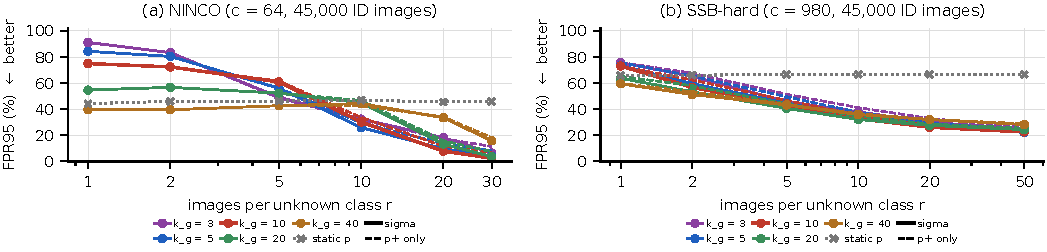
\includegraphics[width=\textwidth]{figs/fig18_kg.pdf}
\caption{近傍数$k_g$を変えた再出現の格子（\FPR{}，単体，DINOv2 L/14 + DINOv3 L/16）．実線は$\sigma$，破線は$\pP$だけ，灰色の点線は静的$p$（$k_g$に依らない）．}
\label{fig:kg}
\end{figure*}

\section{種の上限$\tau$の格子}
\label{sec:app_cap}
\tabref{caprec}に，\secref{cap}の上限付きの規則を\secref{rec}の格子の全条件で評価した\FPR{}を示す（単体，3回の平均）．混入率が低い条件ではStorey型の閾値が$\tau$に達せず，上限付きと上限なしの値は一致する．混入率30\%以上の\NCaprecNHi{}条件（SSB-hard 980クラス$\times$20，50枚）では上限付きのStorey型は$\pP$だけより\NCaprecStoreycHiMaxMinusLpAbs{}--\NCaprecStoreycHiMinMinusLpAbs{}ポイント良く，980クラス$\times$50枚では種に混じるIDの割合が\NCaprecSsbHardCNineEightZeroRFiveZeroStoreyIdfrac{}から\NCaprecSsbHardCNineEightZeroRFiveZeroStoreycIdfrac{}に下がる．全\NCaprecNCells{}条件で上限付きのStorey型が$\pP$だけより1ポイント以上悪いのは\NCaprecStoreycAllNWorseLpOne{}条件（NINCO $c{=}10,20$の$r{=}10$；上限なしも同じ値）で，そこでは種が数十枚しか選ばれず，その\NCaprecNincoCOneZeroROneZeroStoreycIdfracPct\%がIDである（未知がごく少なく$\hat\pi_0$が小さく出る条件；単純BH法は種を選ばない）．単純BH法は上限の有無に依らず全条件で$\pP$だけより最大\NCaprecBhcAllMaxMinusLp{}ポイントしか悪くならない．登録時の仮説H3（付録\ref{sec:app_hyp}：混入率30\%以上で$\pP$だけより1ポイント以上悪くならず，$r\ge10$・混入率30\%未満で上限なしの利得を1ポイント以内に保つ）は，後者の\NCaprecLoROneZeroN{}条件での差が最大\NCaprecLoROneZeroMaxStoreycMinusStorey{}ポイントであり，成り立つ．


\begin{table*}[t]
\centering
\caption{種の上限$\tau{=}0.05$の規則の格子（\FPR{}[\%]，単体，3回の平均）．Storey型・単純BH法はそれぞれ上限なし／あり．種はDINOv3 L/16のビューで上限付きStorey型に選ばれた枚数（2つの折の合計）とそのうちIDの割合（\%）．}
\label{tab:caprec}
\vspace{1.5mm}
{\fontsize{6.3pt}{7.4pt}\selectfont\renewcommand{\arraystretch}{1.0}%
\setlength{\tabcolsep}{2.2pt}\begin{tabular}{@{}rrr|cc|cc|c|c|cc@{}}
\hline
\rule[-2.0pt]{0pt}{8.2pt} & & & \multicolumn{2}{c|}{Storey型} & \multicolumn{2}{c|}{単純BH法} & & & \multicolumn{2}{c}{種（上限付きStorey型）} \\
\rule[-2.0pt]{0pt}{8.2pt}$c$ & $r$ & 混入率 & 上限なし & $\tau{=}0.05$ & 上限なし & $\tau{=}0.05$ & $\pP$のみ & 静的$p$ & 枚数 & ID \\
\hline
\multicolumn{10}{@{}l}{\rule{0pt}{6.6pt}\textit{NINCO}} \\
5 & 1 & 0.0 & 73.3 & 73.3 & 73.3 & 73.3 & 73.3 & 33.3 & 0 & -- \\
5 & 2 & 0.0 & 76.7 & 76.7 & 76.7 & 76.7 & 76.7 & 63.3 & 0 & -- \\
5 & 5 & 0.1 & 76.0 & 76.0 & 76.0 & 76.0 & 76.0 & 46.7 & 0 & -- \\
5 & 10 & 0.1 & 40.7 & 40.7 & 40.7 & 40.7 & 40.7 & 69.3 & 35 & 81.9 \\
5 & 20 & 0.2 & 11.7 & 11.7 & 9.7 & 9.7 & 10.7 & 43.3 & 91 & 71.2 \\
5 & 30 & 0.3 & 10.9 & 10.9 & 12.0 & 12.0 & 14.4 & 34.2 & 189 & 58.8 \\
10 & 1 & 0.0 & 73.3 & 73.3 & 73.3 & 73.3 & 73.3 & 33.3 & 0 & -- \\
10 & 2 & 0.0 & 78.3 & 78.3 & 78.3 & 78.3 & 78.3 & 55.0 & 0 & -- \\
10 & 5 & 0.1 & 70.7 & 70.7 & 70.7 & 70.7 & 70.7 & 52.7 & 0 & -- \\
10 & 10 & 0.2 & 28.7 & 28.7 & 26.7 & 26.7 & 26.7 & 45.7 & 70 & 79.1 \\
10 & 20 & 0.4 & 8.8 & 8.8 & 10.0 & 10.0 & 10.7 & 39.2 & 232 & 53.8 \\
10 & 30 & 0.7 & 1.4 & 1.4 & 2.0 & 2.0 & 4.9 & 35.1 & 436 & 50.3 \\
20 & 1 & 0.0 & 60.0 & 60.0 & 60.0 & 60.0 & 60.0 & 35.0 & 0 & -- \\
20 & 2 & 0.1 & 77.5 & 77.5 & 77.5 & 77.5 & 77.5 & 40.0 & 0 & -- \\
20 & 5 & 0.2 & 68.0 & 68.0 & 68.0 & 68.0 & 68.0 & 45.7 & 0 & -- \\
20 & 10 & 0.4 & 36.2 & 36.2 & 34.7 & 34.7 & 34.7 & 44.5 & 35 & 71.7 \\
20 & 20 & 0.9 & 9.0 & 9.0 & 8.5 & 8.5 & 11.8 & 52.5 & 415 & 46.1 \\
20 & 30 & 1.3 & 3.9 & 3.9 & 4.3 & 4.3 & 6.9 & 45.6 & 955 & 48.8 \\
40 & 1 & 0.1 & 75.8 & 75.8 & 75.8 & 75.8 & 75.8 & 47.5 & 0 & -- \\
40 & 2 & 0.2 & 70.8 & 70.8 & 70.8 & 70.8 & 70.8 & 46.2 & 0 & -- \\
40 & 5 & 0.4 & 67.8 & 67.8 & 67.8 & 67.8 & 67.8 & 46.5 & 0 & -- \\
40 & 10 & 0.9 & 35.2 & 35.2 & 34.5 & 34.5 & 34.5 & 48.9 & 175 & 58.5 \\
40 & 20 & 1.7 & 9.8 & 9.8 & 10.2 & 10.2 & 12.9 & 49.8 & 1081 & 47.5 \\
40 & 30 & 2.6 & 2.7 & 2.7 & 3.2 & 3.2 & 5.9 & 45.1 & 1766 & 41.5 \\
64 & 1 & 0.1 & 75.0 & 75.0 & 75.0 & 75.0 & 75.0 & 44.3 & 0 & -- \\
64 & 2 & 0.3 & 72.4 & 72.4 & 72.4 & 72.4 & 72.4 & 46.1 & 0 & -- \\
64 & 5 & 0.7 & 60.9 & 60.9 & 61.6 & 61.6 & 61.6 & 46.2 & 33 & 74.5 \\
64 & 10 & 1.4 & 30.2 & 30.2 & 30.5 & 30.5 & 33.7 & 46.9 & 296 & 46.2 \\
64 & 20 & 2.8 & 7.9 & 7.9 & 7.7 & 7.7 & 11.7 & 45.5 & 1689 & 41.5 \\
64 & 30 & 4.1 & 2.5 & 2.5 & 2.9 & 2.9 & 6.7 & 46.0 & 2664 & 36.6 \\
\multicolumn{10}{@{}l}{\rule{0pt}{6.6pt}\textit{SSB-hard}} \\
10 & 1 & 0.0 & 90.0 & 90.0 & 90.0 & 90.0 & 90.0 & 66.7 & 0 & -- \\
10 & 2 & 0.0 & 86.7 & 86.7 & 86.7 & 86.7 & 86.7 & 73.3 & 0 & -- \\
10 & 5 & 0.1 & 82.0 & 82.0 & 82.0 & 82.0 & 82.0 & 53.3 & 0 & -- \\
10 & 10 & 0.2 & 60.0 & 60.0 & 60.0 & 60.0 & 60.0 & 63.3 & 0 & -- \\
10 & 20 & 0.4 & 45.8 & 45.8 & 47.0 & 47.0 & 46.8 & 69.8 & 122 & 64.8 \\
10 & 50 & 1.1 & 11.5 & 11.5 & 11.1 & 11.1 & 18.1 & 65.7 & 535 & 48.5 \\
30 & 1 & 0.1 & 71.1 & 71.1 & 71.1 & 71.1 & 71.1 & 55.6 & 0 & -- \\
30 & 2 & 0.1 & 82.8 & 82.8 & 82.8 & 82.8 & 82.8 & 65.0 & 0 & -- \\
30 & 5 & 0.3 & 79.1 & 79.1 & 79.1 & 79.1 & 79.1 & 65.1 & 0 & -- \\
30 & 10 & 0.7 & 60.7 & 60.7 & 60.3 & 60.3 & 60.3 & 58.9 & 72 & 77.0 \\
30 & 20 & 1.3 & 43.3 & 43.3 & 43.5 & 43.5 & 46.4 & 71.0 & 344 & 51.4 \\
30 & 50 & 3.2 & 16.5 & 16.5 & 16.3 & 16.3 & 25.1 & 67.3 & 1507 & 41.9 \\
100 & 1 & 0.2 & 80.0 & 80.0 & 80.0 & 80.0 & 80.0 & 65.0 & 0 & -- \\
100 & 2 & 0.4 & 84.0 & 84.0 & 84.0 & 84.0 & 84.0 & 71.0 & 0 & -- \\
100 & 5 & 1.1 & 76.1 & 76.1 & 75.8 & 75.8 & 75.8 & 70.3 & 33 & 87.9 \\
100 & 10 & 2.2 & 50.7 & 50.7 & 51.5 & 51.5 & 56.5 & 68.1 & 404 & 55.2 \\
100 & 20 & 4.3 & 32.4 & 32.4 & 33.3 & 33.3 & 38.5 & 66.9 & 1597 & 44.2 \\
100 & 50 & 10 & 18.5 & 18.5 & 18.7 & 18.7 & 24.2 & 67.2 & 5132 & 31.6 \\
300 & 1 & 0.7 & 78.6 & 78.6 & 78.6 & 78.6 & 78.6 & 67.1 & 0 & -- \\
300 & 2 & 1.3 & 73.6 & 73.6 & 73.6 & 73.6 & 73.6 & 64.7 & 0 & -- \\
300 & 5 & 3.2 & 58.9 & 58.9 & 58.7 & 58.7 & 62.2 & 64.6 & 402 & 49.7 \\
300 & 10 & 6.2 & 42.3 & 42.3 & 42.8 & 42.8 & 47.9 & 66.8 & 1751 & 38.0 \\
300 & 20 & 12 & 29.7 & 29.7 & 29.9 & 29.9 & 34.2 & 65.7 & 5348 & 32.2 \\
300 & 50 & 25 & 19.3 & 19.6 & 19.6 & 19.6 & 22.1 & 66.9 & 14736 & 19.1 \\
980 & 1 & 2.1 & 73.1 & 73.1 & 72.9 & 72.9 & 72.9 & 65.9 & 33 & 84.7 \\
980 & 2 & 4.2 & 56.8 & 56.8 & 56.5 & 56.5 & 62.4 & 66.1 & 522 & 47.5 \\
980 & 5 & 9.8 & 43.1 & 43.1 & 42.7 & 42.7 & 46.7 & 66.6 & 3381 & 36.1 \\
980 & 10 & 18 & 32.8 & 32.8 & 32.6 & 32.6 & 35.5 & 66.7 & 9372 & 31.0 \\
980 & 20 & 30 & 26.2 & 26.1 & 26.1 & 26.1 & 27.8 & 66.8 & 17485 & 16.7 \\
980 & 50 & 52 & 22.6 & 22.2 & 21.5 & 22.2 & 23.4 & 66.6 & 40958 & 6.6 \\
\hline
\end{tabular}}%

\end{table*}

\section{追加実験の事前登録と仮説の判定}
\label{sec:app_hyp}
\secref{cap}の上限付きの種，\secref{in200}の全学習画像・ゼロショットの基線，付録\ref{sec:app_kg}の$k_g$の格子，付録\ref{sec:app_views}の中心化は，1つの登録文書（公開リポジトリの\texttt{experiments/phase15/prereg\_p15.json}，SHA-256 \texttt{83ea4061}$\cdots$）に計算の内容・報告の形・6つの仮説を記してから実行した．登録文書は評価の実行前に公開リポジトリのブランチ\texttt{phase12-15-registrations}（コミット\texttt{8ef9c8d}）にコミットし，その時刻が第三者の確認できる時刻である（学習画像の特徴抽出だけはコミット前に始めた）．構成の選択は行わず（$\tau$と$q$は固定，本稿の主構成は変えない），登録からの逸脱はない．系1の実測（付録\ref{sec:app_kg}）は査読後に加えた登録外の記述的な計算で，選択を含まない．判定は次のとおりである．
\textbf{H1}（上限は害を消す：CIFAR-100 far-OODとImageNet-200 near-OODで上限付きの規則は$\pP$だけの+0.5ポイント以内）：成立（+\NCifarStoreycFarDfprVsLp{}，\NInTwoZeroZeroStoreycNearDfprVsLp{}ポイント）．
\textbf{H2}（上限はImageNet-1K near-OODで上限なしの0.5ポイント以内）：成立（単体\NCapStoreycAloneNearDfprVsStorey{}，$\times$TINS +\NCapStoreycNearDfprVsStorey{}ポイント）．
\textbf{H3}（格子：混入率30\%以上で$\pP$だけより1ポイント以上悪くならず，$r\ge10$・混入率30\%未満で上限なしの利得を1ポイント以内に保つ）：成立（付録\ref{sec:app_cap}）．
\textbf{H4}（全学習画像のkNN（$k{=}50$）は両ベンチマークで16枚の静的$p$より良く，ImageNet-200のnear-OODでは$\sigma$がkNNより低い\FPR{}を保つ）：前半は否定（ImageNet-200でkNN \NInTwoZeroZeroKnnAllKFiveZeroNearFpr\%／\NInTwoZeroZeroKnnAllKFiveZeroFarFpr\%対静的$p$ \NInTwoZeroZeroStaticNearFpr\%／\NInTwoZeroZeroStaticFarFpr\%，CIFAR-100のfar-OODで\NCifarKnnAllKFiveZeroFarFpr\%対\NCifarStaticFarFpr\%；CIFAR-100のnear-OODだけ\NCifarKnnAllKFiveZeroNearFpr\%対\NCifarStaticNearFpr\%），後半は成立（\NInTwoZeroZeroMainNearFpr\%対\NInTwoZeroZeroKnnAllKFiveZeroNearFpr\%）．
\textbf{H5}（$\sigma$が静的$p$を下回る$r$は$k_g$が小さいほど小さく，大きい$r$での利得は$k_g\in\{10,20\}$で最大）：前半は否定，後半は$\{5,10\}$として部分的に成立（付録\ref{sec:app_kg}）．
\textbf{H6}（中心化でCLIPの静的$p$はDINO系の範囲（near 70\%未満，far 40\%未満）に入り，DINO系の変化は10ポイント以内）：前半は否定（near \NViewClipStaticcNearFpr\%，far \NViewClipStaticcFarFpr\%），後半は静的$p$で成立（最大\NViewsDinoCentredMaxabsFpr{}ポイント），kNNではDINO (v1)のfar-OODで\NViewsDinoKnncentredMaxabsFpr{}ポイント動く．
